%
% File: chap03.tex
% Author:
% Description: Design and Implementations
%
\chapter{Methodology}
\label{chap:D&I}

\section{Work Flow}
\label{subsec:subsec01}

\section{Project Management}
\label{subsec:PM}
\input{ProjectManagement.tex}

\section{Front-end Tools}
\label{subsec:FETools}
%
% File: chap03-01-02.tex
% Author: 
% Description: 
% 3.1 Methodology
%  3.1.2 Front-end Tools
%     Figma
%     HTML
%     CSS
%     SpringBoot+Thymeleaf
%

\paragraph{Figma}\mbox{}\\
In our project, our goal is to design a website for medical use. As a team, we all agree that a high-quality website should include several essential factors. Among them, user interface (UI) and user experience (UX) are the most crucial. A well-designed website should maintain a consistent and visually appealing style across all pages, while also being intuitive to use and free from confusing workflows. Another key consideration is the design process itself. Since we are working as a team, it is important to choose a tool and workflow that supports efficient collaboration. First, team members should be allowed to work independently or collaboratively while still ensuring consistency across design. Second, we need a real-time collaborative environment to prevent any individual’s progress from being delayed by others. 

For achieving our project goals, we evaluate two tools, Canva and Figma. Both are useful for collaborative website development and support real-time commenting to improve teamwork. However, the key differences lie in several areas. First is layout design. Figma allows for the detailed design of every element on each page, including font size and CSS box models. In contrast, Canva cannot adjust all elements individually and focuses more on overall visual design. Second is interactive prototyping. Figma features in demonstrating the website’s workflow by allowing us to define the behavior of elements like buttons and links to fully simulate the website experience. Canva, on the other hand, can only create simple links between pages. Third is version control. Figma automatically records a comprehensive history of all changes, while Canvas offers relatively basic version control functions. Ultimately, Figma is our final choice for this project because it provides all the features we need for professional web development.

As our final decision, Figma improved our work due to these features:
\begin{itemize}
    \item \textbf{Real-time Collaboration and Efficiency}: Figma enabled us to work simultaneously in the cloud, with live editing and immediate feedback eliminating unnecessary back-and-forth communication. This transparency allowed everyone to see ongoing progress, making it easier to coordinate tasks and iterate on designs much faster.
    \item \textbf{Guaranteed Visual Consistency}: By utilizing shared elements, colors, and font styles, we successfully maintained a coherent and consistent visual language across the entire interface.
    \item \textbf{Streamlined Development Handoff}: One of the most practical benefits was the automatic generation of CSS code for design properties. This feature greatly enhanced our efficiency by simplifying the process of translating designs into front-end code.
    \item \textbf{Clear Accountability and Version Control}: The ability to tag team members in comments kept us aligned on assigned sections. Furthermore, the comprehensive version control function provided a clear history of all changes, ensuring accountability and allowing us to review progress at any stage.
    \item \textbf{Fostered Collaborative Ownership}: Ultimately, Figma didn't just reduce confusion and latency; it fostered a strong sense of shared ownership over the design. It ensured that our team worked as a cohesive unit, building a product with a unified vision.
\end{itemize}

\paragraph{HTML}\mbox{}\\
We aim to provide a clean, accessible and responsive interface for medical users. To achieve this goal, we requires tools that help us build structured, semantic layouts while maintaining visual consistency across devices and screen sizes. When evaluating which front-end tools were most suitable for our design, we considered several combinations, including HTML with Bootstrap, HTML with TailwindCSS, and SCSS-based modular design systems. According to the specific characteristics of our project and our situation. We all agree that using HyperText Markup Language(HTML) and Cascading Style Sheets(CSS) was the most appropriate choice for our needs after discussion. In the following section, we provide a brief introduction to these two technologies and explain how they contributed to the development of our prototype.

HTML is a necessary and standard core language that can be interpreted by any modern web browsers. In web development, HTML is used to arrange the content of the website and provide basic structural syntax for page design. As a fundamental tool, HTML has a relatively simple and easy-to-learn syntax, allowing developers to create websites with clear semantic structures that enhances both accessibility and user-friendliness. HTML wild ranges of labels, such as \verb|<head>|, \verb|<p>|, and \verb|<div>|, which are used to organise the layout of a page. These elements support essential functions like hyperlinks, image embedding, list creation and tables formatting. With just basic syntax, developers can easily achieve a certain level of responsive functionality. Although various tools exists to assist in web development—such as page builders or frameworks—all of them ultimately compile down to HTML. As a result, HTML is irreplaceable in the front-end development process. Due to the situation our team has encountered, we all agree that the cost of learning alternative tools would beyond their benefits. Therefore, we decide to directly use plain HTML as our primary front-end tool. However, as mentioned above, HTML only provides basic structure and limiting styling capabilities. Managing layout and appearance directly within HTML would lead to inefficiencies and inconsistency. To address this issue, we employed CSS to handle visual design and layout, which will be discussed in next section. 

\paragraph{CSS}\mbox{}\\
One crucial issue in web development is how to manage code efficiently and make it maintainable. A widely adopted and effective solution is to separate the content, functionality and the style into distinct layers. While tools such as SCSS, Tailwind CSS and Bootstrap provide advanced styling features, we ultimately chose to use standard CSS for this project. This decision was based on the simplicity and clarity that CSS provides--especially valuable for a small team working on a focused prototype. CSS allows us to directly translate our Figma designs into code without introducing additional syntax or dependencies. This made it easier for all team members to understand and contribute to the styling process. Besides, one of the key advantages of CSS is its clear separation of content and presentation, which improves maintainability and enables us to update visual styles without modifying the fundamental structure. CSS also plays a crucial role in transforming our HTML structure into a clean, professional, and user-friendly interface. Furthermore, CSS enhances our collaboration by allowing us to define a shared layout and style system. Each members can easily apply consistent styles across pages, significantly reducing time spent on detail adjustments, and improving the efficiency of our workflow.

\paragraph{Spring Boot and Thymeleaf}\mbox{}\\
Before selecting our technology stack for the Smart Hospital web application, we weighed a number of backend and frontend framework possibilities with consideration of equating development speed, maintainability, and integration efficiency. The top contenders included Spring Boot with Thymeleaf, Node.js with Express and React, and Django with HTML templates. Table~\ref{tab:3-1-2-SBtable} summarizes the strengths and weaknesses of each stack based on thoroughly documented pros and cons according to credible sources.

\begin{table}[H]
  \centering
  
\includegraphics[width=0.8\linewidth]{images03/3-1-2-springbootTable.png} 
  \caption{Technology Stack Alternatives Comparison}
  \label{tab:3-1-2-SBtable}
\end{table}

We weighed these options and opted to go with Spring Boot in the backend and Thymeleaf in the frontend. This Java-focused stack provided us with a consistent and streamlined development environment, which was particularly crucial for our small team of individuals working on tight deadlines. Because both frameworks are based on the Java ecosystem, we were able to build full-stack functionality in one integrated project. This reduced the complexity that would have otherwise been caused by having two separate frontend and backend codebases and improved coordination among team members.\cite{Simplilearn-Nodejs-SB}

Spring Boot is a well-used enterprise-level framework that streamlines Java web application development. It provides an embedded Tomcat server, auto-configuration, and dependency management, allowing us to concentrate on core functionality instead of boilerplate setup.\cite{GFG-Djanggo-SB} Its innate RESTful API support enabled us to plan a scalable, modular backend architecture, with Controller classes as the basis for API endpoints, a core feature for connecting the client interface to backend services.

At the frontend, Thymeleaf was selected as a server-side templating engine that has native support for Spring Boot's MVC framework. Its dynamic binding of backend data in HTML templates ensured tight coupling of presentation logic with backend processes. This eliminated the need for extra JavaScript frameworks like React or Angular, reducing the learning curve and allowing the team to progress faster. Thymeleaf's human-readable syntax also made collaboration easier and the codebase more maintainable.\cite{JavaGuides-Thymeleaf-ReactJS}

Alternatives such as Node.js with Express and React were also considered, which would have offered highly interactive UIs and would have leveraged JavaScript's extensive ecosystem, but would also have meant two codebases to manage and deployment complexity.\cite{Simplilearn-Nodejs-SB} Django with HTML templates, knowingly able to achieve rapid development and secure by design \cite{GFG-Djanggo-SB}, was also a consideration but would have required the team to learn Python, an undesirable learning curve considering the time constraints we had.

Finally, our academic supervisor recommended picking up Spring Boot with Thymeleaf for its combination of performance, integration ease, and suitability for a Java-experienced team. This also simplified deployment, as both backend and frontend could be deployed together in a single application. Moving further to the backend implementation phase, Spring Boot Controller classes will accept incoming HTTP requests and will form the basis of our API layer, which, later on, will be tested by tools discussed in the Backend Tools section.


\section{Back-end Tools}
\label{subsec:BETools}
\paragraph{Programming Language}\mbox{}\\
There are three main programming languages we considered for the backend: Java, Python, and C. Most of us had just finished the Object-Oriented Programming with Java module, so Java is familiar and quick to pick up for us. C is a high-performance language, and we had also learned it in our first-semester Programming in C course, but manual memory management and the lack of higher-level web frameworks would slow us down and increase maintenance risk. The last language considered was Python. It is good for fast prototyping, but our experience was uneven—some team members had never even used it before. Under time pressure, it would be quite challenging for all of us to learn and effectively use it.

We therefore chose Java with Spring Boot. Java's static typing and compile-time checks help us model clinical data more safely. Spring provides built-in support for REST endpoints and data access, and Maven keeps builds simple. This stack let us deliver features steadily within the course schedule.


\section{Testing Tools}
\label{subsec:subsec05}

\chapter{Front-end Design and Implementations}
\label{sec:sec02}

\section{Early Stage-Virtual Hospital Africa(VHA)}
\label{subsec:subsec01}
%
% File: chap03-02-01.tex
% Author:
% Description:
% 3.2 Front-end Design & Implementation
%  3.2.1 Early Stage-Virtual Hospital Africa(VHA)
%
%

\paragraph{Design Process}\mbox{}\\
During initial discussions with the client about their requirements, the client pointed out that the current website's Patient Intake page contained too many information fields, leading to poor user experience and even many testers abandoning the form midway during testing (Figure 3.1). Based on this situation, the client designed a second version of the multi-step form interface (Figure 3.2). The original form was split into separate pages (personal information, contact information, primary care, reason for visit), each with a progress indicator to guide users through the process.

During the programming and testing of the second version design, group members identified several issues that could potentially impact usability in actual interactions. We conducted internal team discussions and shared these issues with the client during our weekly design meetings. Ultimately, the client adopted our suggestions and finalized the third version design (Figure 3.3), with the following key improvements:

\begin{itemize}
    \item 1. Added a left-side navigation bar to enable non-linear navigation
\end{itemize}
The original design relied solely on the top progress bar, requiring users to complete steps in a fixed order. We suggested adding a modular navigation bar on the left side, allowing users to freely jump to any section for modifications, thereby enhancing their sense of control and flexibility \cite{nielsen1995}.

\begin{itemize}
    \item 2. Optimized field grouping and information hierarchy
\end{itemize}
We consolidated information such as name, gender, title, language, and national ID number into the “General” group and introduced a profile photo upload function on this page to add a patient profile photo capture/upload feature. This aligns the website's information layout with users' real-world information collection habits and aligns with the standard practice in hospital admission processes of “first collecting basic information and taking photos for record-keeping.” Additionally, once the avatar upload is complete, a preview will be displayed immediately, and the centralized presentation of related fields will allow users to quickly confirm the accuracy of key information in a unified area, ensuring visibility of the interaction process \cite{nielsen1995}.

\begin{itemize}
    \item 3. Unify navigation button layout
\end{itemize}
In the third version design, since we removed the top global navigation bar, users need clearer prompts for the next steps in the interface. Based on Nielsen's (1995) usability principles of “Visibility of system status” and “Match between system and the real world,” we replaced the bottom buttons with ‘Back’ and “Next” as alternative navigation methods, clearly indicating the user's forward and return paths. This design reduces users' sense of disorientation during task flows, enhances the predictability of operations, and increases the certainty of task completion.

Regarding the second group: The client's requirements primarily focused on the patient profile page, highlighting several shortcomings in the current interface regarding information presentation and user experience. These include lack of detailed patient identification methods and information, absence of quick access points, unclear information structure, absence of direct editing functions, low efficiency in switching between information modules, and insufficient visual hierarchy in the interface (Figure 3.4). In response to the client's requirements, we proposed several improvement suggestions, which were confirmed in subsequent meetings with the client, ultimately resulting in the design of the new version (Figure 3.5):

\begin{itemize}
    \item 1. Enhance the patient information card: Add a profile picture, gender/age tags, patient status, quick contact button, download patient report button, and last edit time to the patient information card. This not only avoids healthcare staff having to make additional clicks or page switches to confirm patient identity and status but also addresses the issue of being unable to perform common operations directly on the patient profile page, enabling quick identification and efficient management of patient information.
    \item 2. Expand the patient information module and optimize the information navigation structure: Introduce more patient information modules in the Patient Profile, unify the naming and order of the top tab bar, and add a secondary menu on the left side, dividing the information into modules such as General, Primary Care, Contacts, Biometrics, and Insurance. This modular structure enhances the completeness of the information, allowing users to efficiently obtain the required data on a single page and reducing the need for frequent page switching or scrolling to find information.
    \item 3. Switch to editable forms: Present personal information in structured fields that support direct editing. This simplifies the information maintenance process, reduces operational steps, and enhances the user experience.
\end{itemize}
The third group of customers' needs were mainly focused on the Vitals page, and they pointed out that the current interface had many shortcomings in terms of data input structure and interaction experience, mainly including: all vital signs items were stacked in a single list, with no clear distinction between required and optional fields, making it difficult for users to quickly identify which fields to fill in first; the order of the fields did not fully match the clinical data collection process, and some commonly used data items were not placed prominently enough; the page lacked step-by-step navigation or process guidance, and users might not be able to confirm their progress(Figure 3.6). After internal discussions, we proposed improvement suggestions for these issues and reached consensus with the client during meetings, ultimately finalizing the new version design (Figure 3.7):

\begin{itemize}
    \item 1. Grouped layout and priority adjustments
\end{itemize}
Vital sign information is divided into two main sections: “Required” and “Optional,” ensuring that healthcare professionals prioritize the collection of critical data; the field order is adjusted to better align with actual clinical data collection practices (e.g., first entering height, weight, temperature, blood pressure, and pulse rate, followed by optional items such as blood glucose, oxygen saturation, and respiratory rate) \cite{webform}.

\begin{itemize}
    \item 2. Optimized operational workflow
\end{itemize}
Added Back/Next navigation buttons at the bottom of the page to replace the original single “Continue” button, allowing users to more intuitively control the progress of form completion and avoid omissions due to skipping or accidental operations.

\begin{itemize}
    \item 3. Integration with patient information panel
\end{itemize}
Retained the patient profile summary and treatment timeline (Seeking Treatment) on the right side, ensuring that healthcare professionals can reference the patient's status and completed examination steps at any time during data entry.

These changes adhere to usability principles such as “Match between system and the real world,” “Visibility of system status,” and “Recognition rather than recall,” reducing cognitive load, improving data entry efficiency, and minimizing operational errors \cite{nielsen1995}.

\begin{figure}[H]
    \centering
    \begin{minipage}{0.47\textwidth}
        \centering
        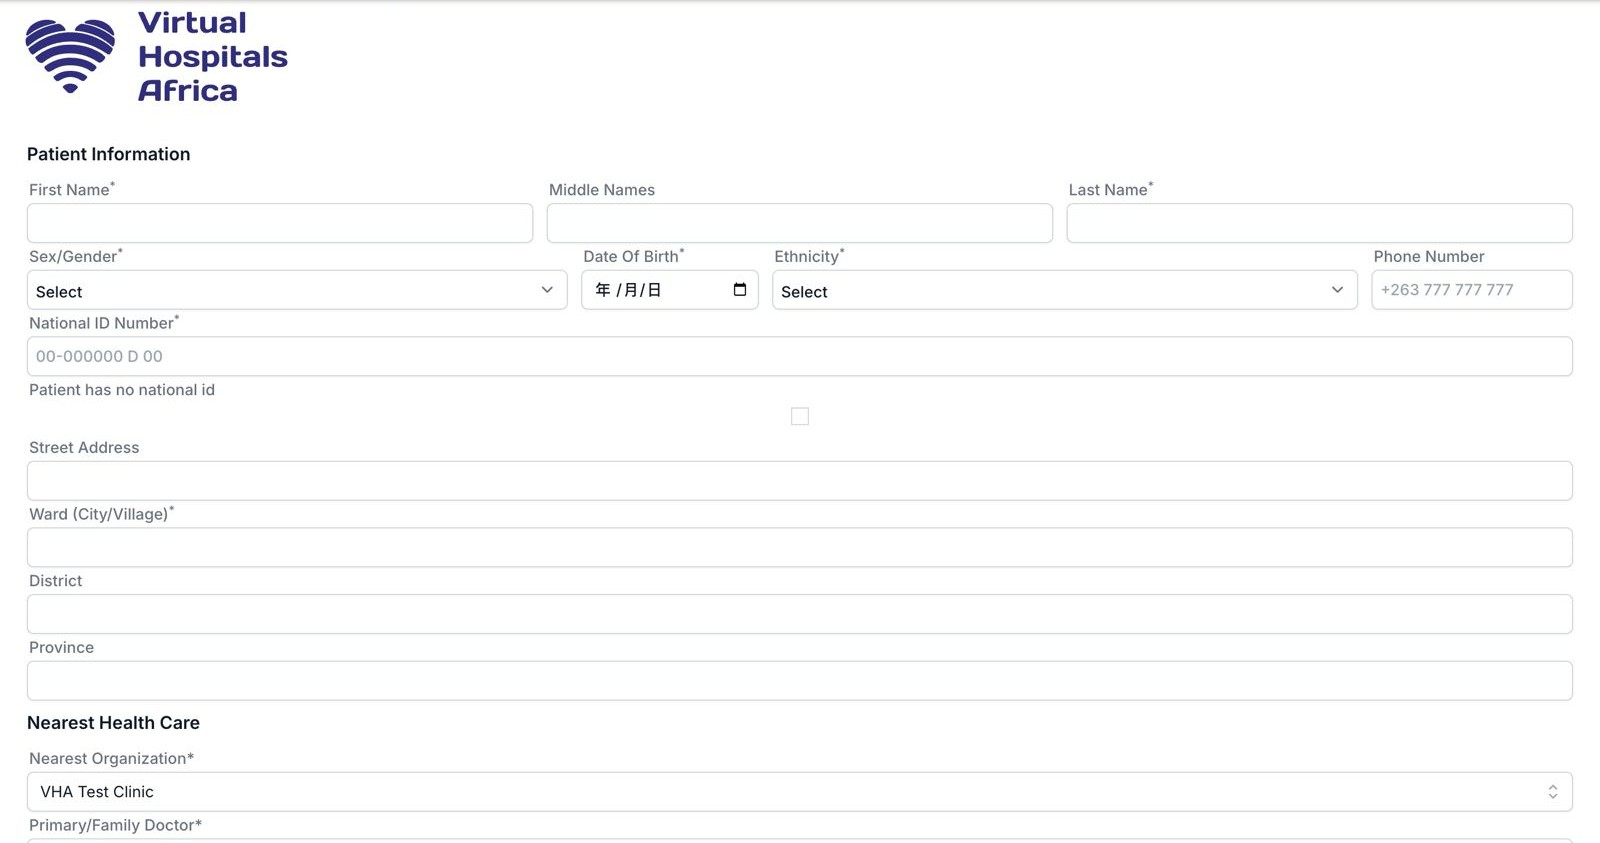
\includegraphics[width=\textwidth]{images/(VHA)-1.jpg}
        \caption{Patient Intake page – original version / user feedback context}
        \label{fig:design-1}
    \end{minipage}\hfill
    \begin{minipage}{0.47\textwidth}
        \centering
        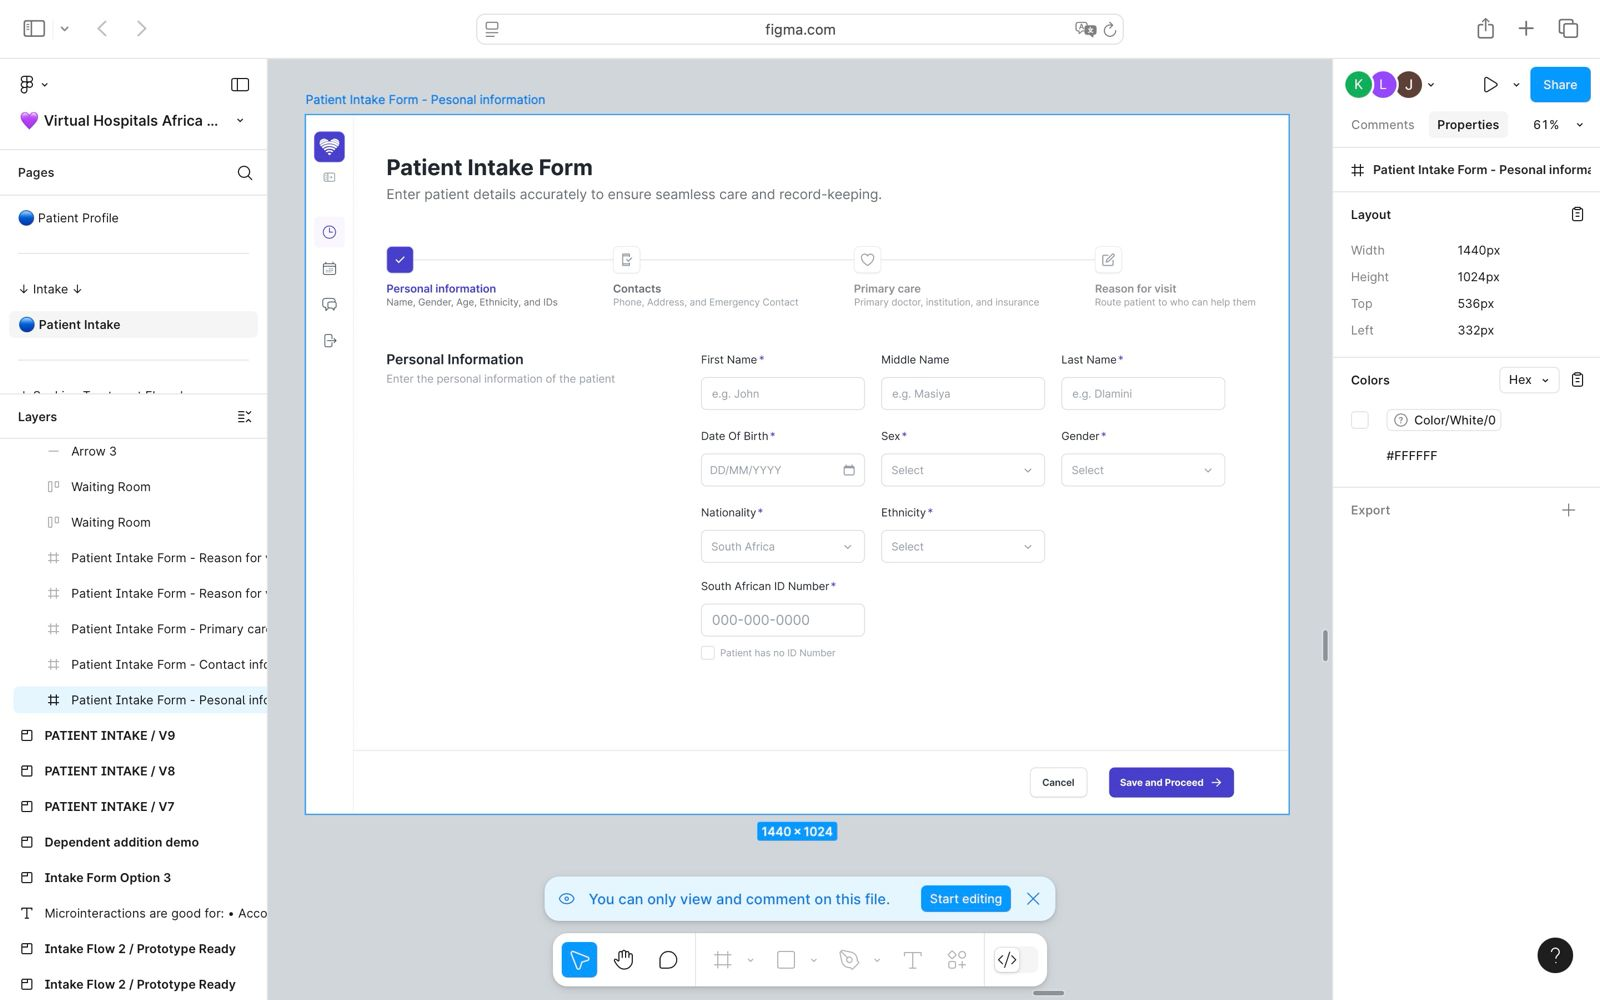
\includegraphics[width=\textwidth]{images/(VHA)-2.jpg}
        \caption{Second version multi-step form interface}
        \label{fig:design-2}
    \end{minipage}
\end{figure}
\begin{figure}[H]
    \centering
    \begin{minipage}{0.47\textwidth}
        \centering
        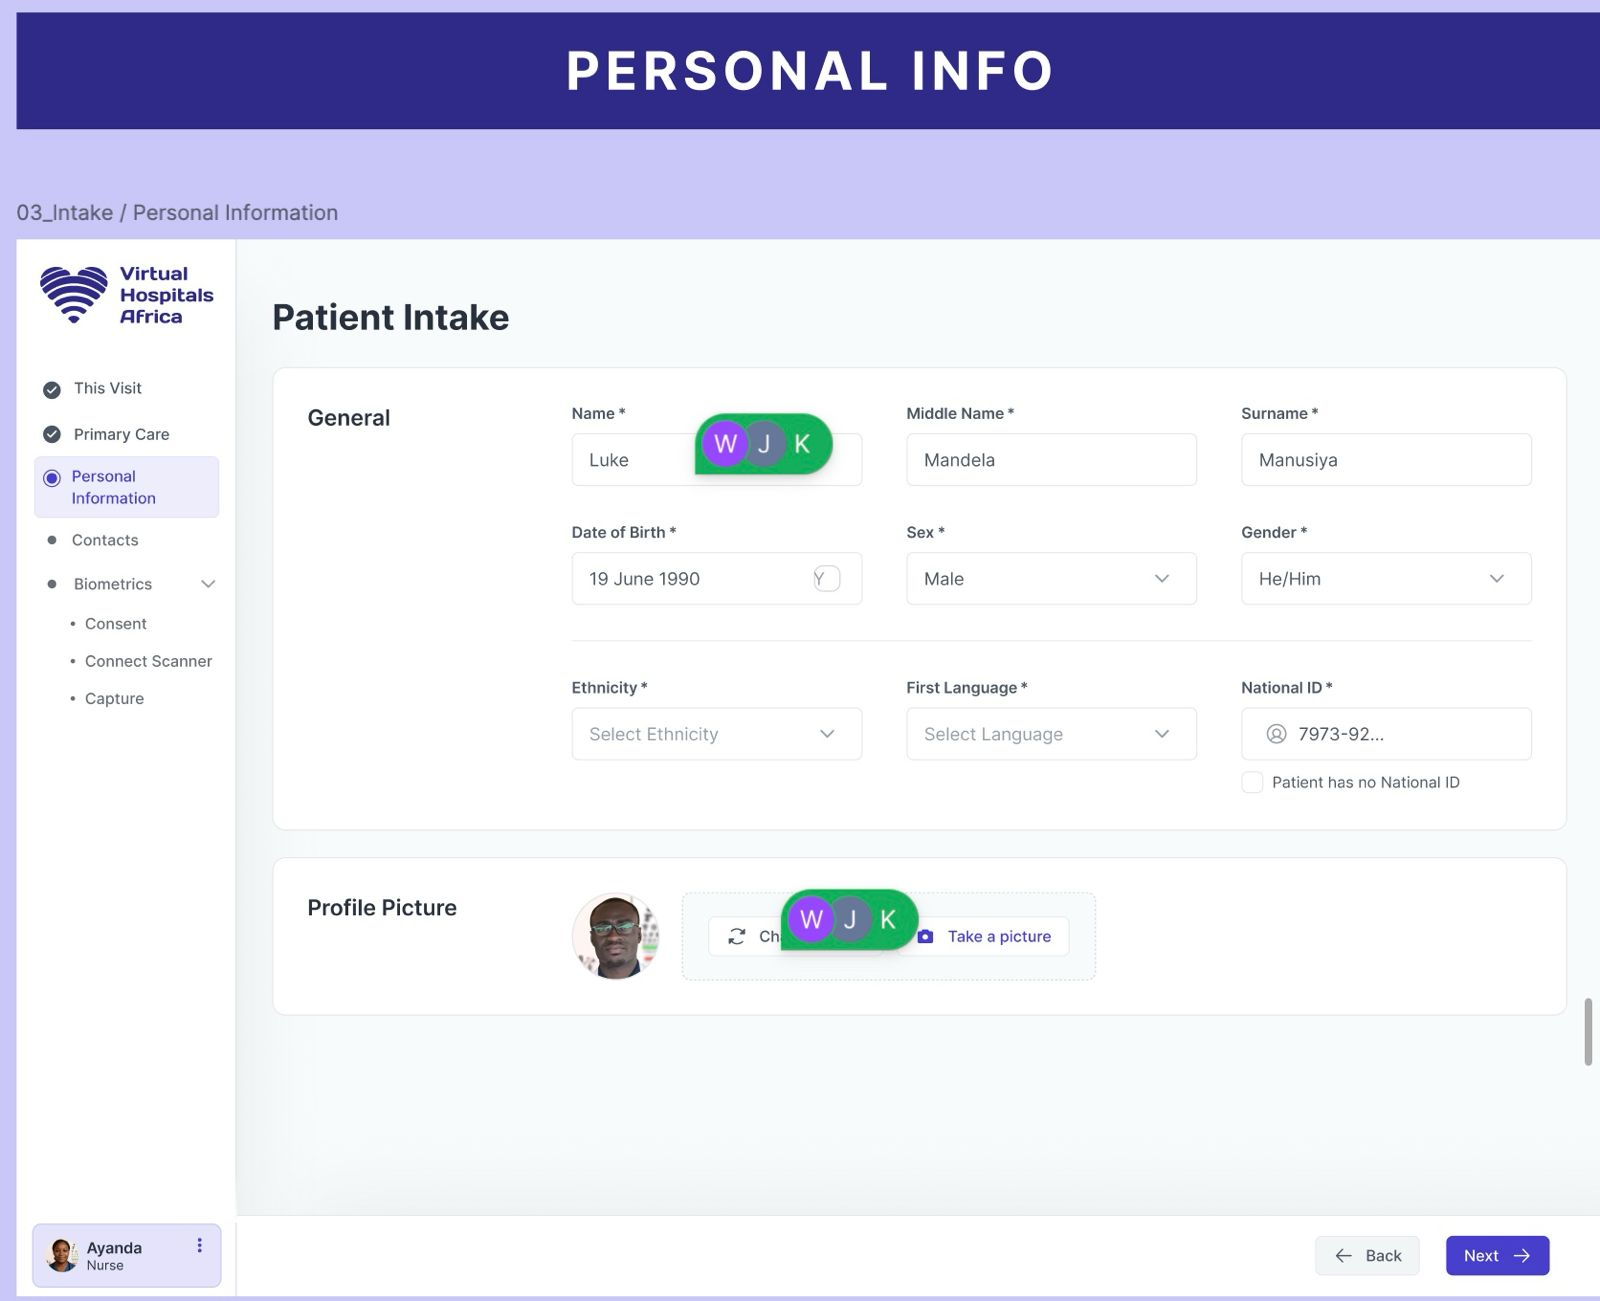
\includegraphics[width=\textwidth]{images/(VHA)-3.jpg}
        \caption{Third version with left-side navigation and unified buttons}
        \label{fig:design-3}
    \end{minipage}\hfill
    \begin{minipage}{0.47\textwidth}
        \centering
        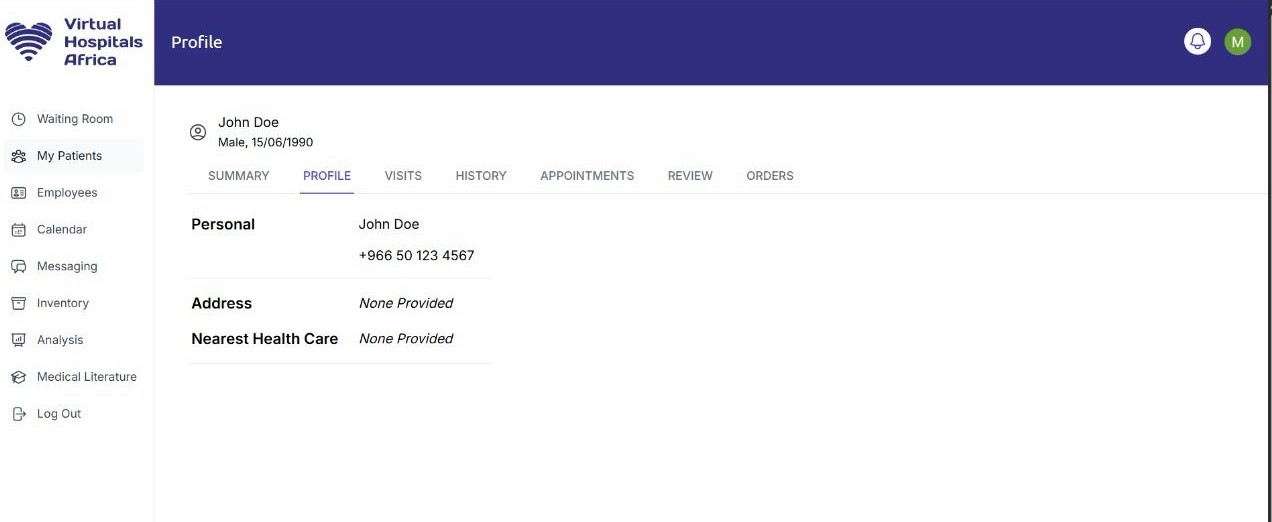
\includegraphics[width=\textwidth]{images/(VHA)-4.jpg}
        \caption{Patient profile page – issues in current interface}
        \label{fig:design-4}
    \end{minipage}
\end{figure}
\begin{figure}[H]
    \centering
    \begin{minipage}{0.47\textwidth}
        \centering
        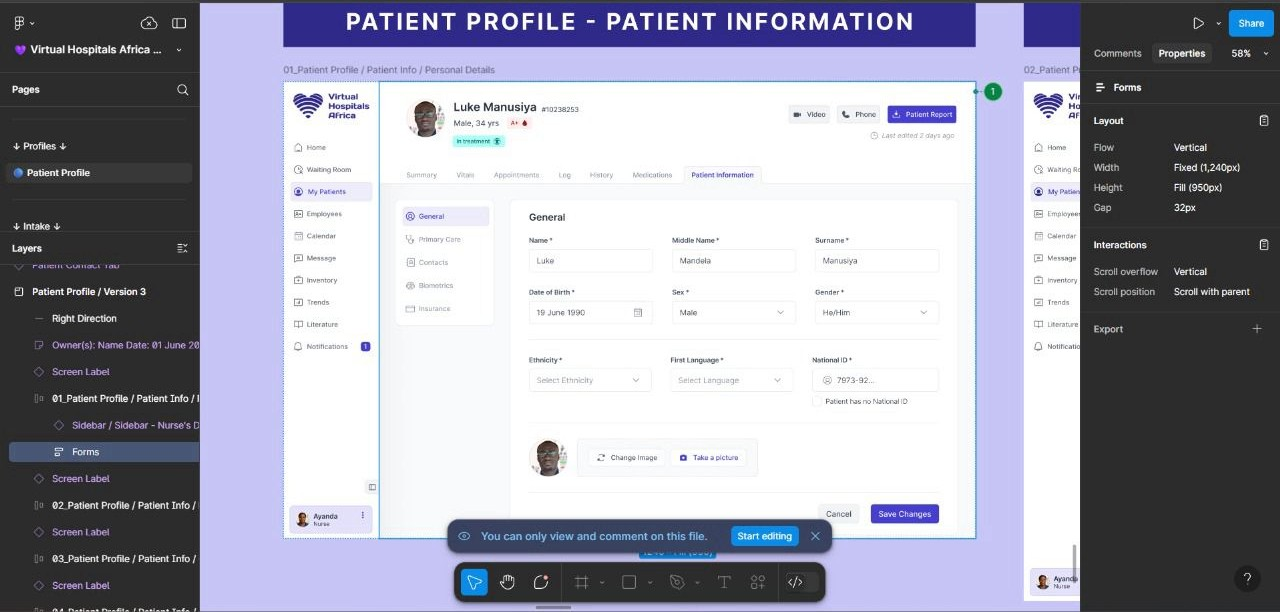
\includegraphics[width=\textwidth]{images/(VHA)-5.jpg}
        \caption{Redesigned patient profile with improved info card and modules}
        \label{fig:desbign-5}
    \end{minipage}\hfill
    \begin{minipage}{0.47\textwidth}
        \centering
        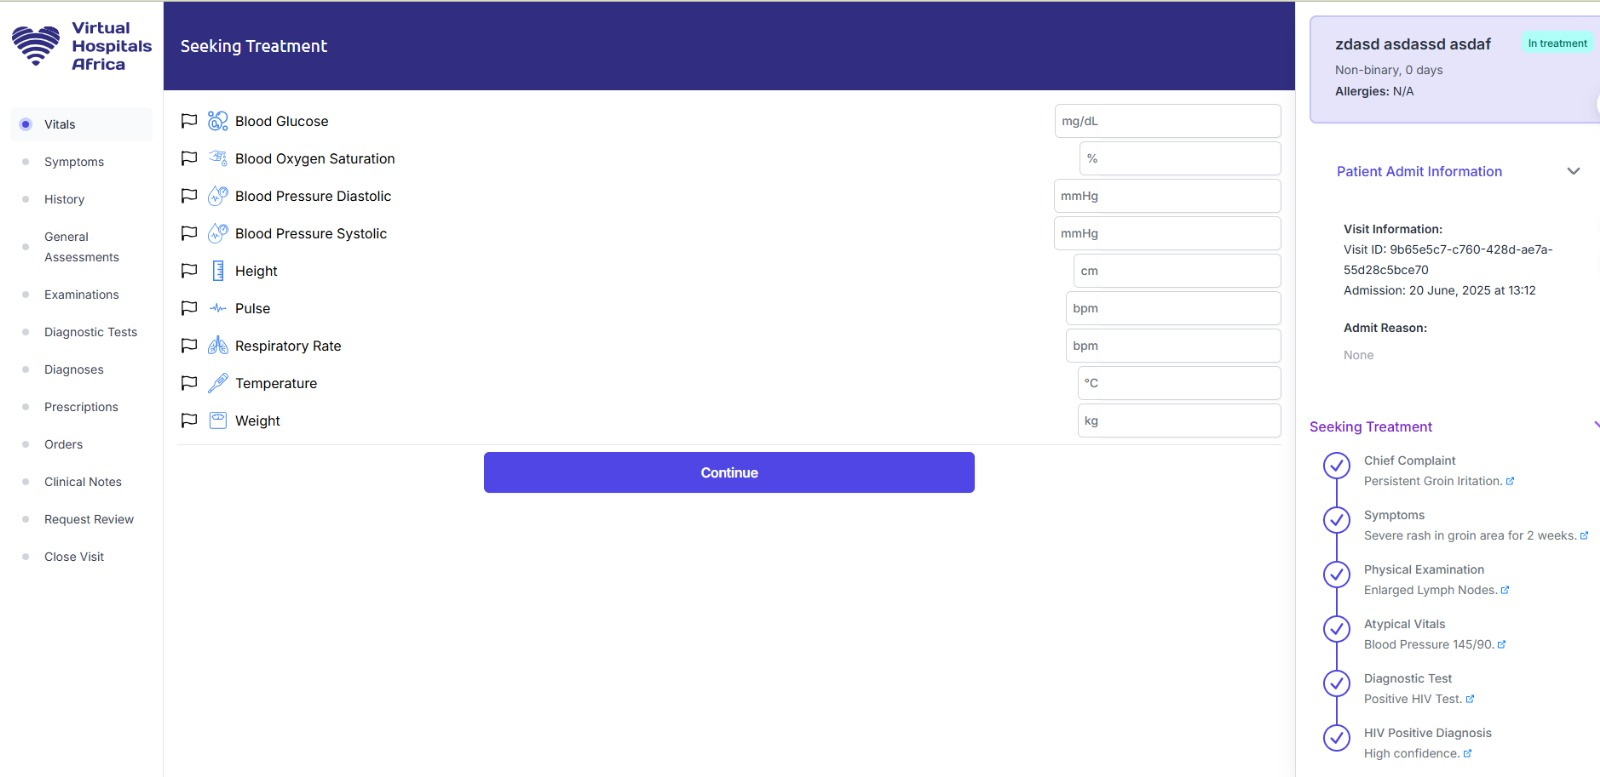
\includegraphics[width=\textwidth]{images/(VHA)-6.jpg}
        \caption{Vitals page – issues in original layout}
        \label{fig:design-6}
    \end{minipage}
\end{figure}

\subsection{Code Implementation - Patient Data Management}

Virtual Hospitals Africa's goal is to implement a virtual hospital website with a fast user interface that is also maintainable and adaptable. Achieved by using type-safe frameworks, such as TypeScript and React, to ensure code quality and reduce runtime errors and the utility first approach with tailwind CSS.

\paragraph{TypeScript}\mbox{}

TypeScript is a superset of JavaScript which allows developers to catch errors at compile time rather than runtime, making it easier to maintain and refactor code. It provides static type checking, which helps in identifying any potential issues early in the development process. This is particularly useful for large codebases like Virtual Hospitals Africa, where maintaining code quality and consistency is crucial. The codebase demonstrates type definitions for complex data structures, as shown in the patient management system components. TypeScript's type system provides significant advantages in large-scale application development by enabling early error detection and improved code maintainability (Bierman et al., 2014).

The implementation showcases strong type safety through interfaces and type definitions. For example, the \texttt{Measurements} definition in \texttt{type.ts} includes precise geographic positioning with \texttt{latitude: number} and \texttt{longitude: number} properties, along with optional \texttt{admit\_reasons?: string[]} arrays. The patient data structure demonstrates TypeScript's nullable type handling with properties like \texttt{age\_years?: Maybe<number> | string | null}, showcasing the framework's flexibility in handling uncertain data states.

The SQL integration in \texttt{patient.ts} demonstrates TypeScript's template literal types and generic constraints with complex database queries: \texttt{\detokenize{sql<string | null>`
\patient_age.age_years::text`.as('age_years')`}} and string interpolation for formatted patient data. This ensures type safety in SQL queries, preventing runtime errors and increasing code reliability.

Interface Segregation Principles (ISP) guide the API contracts and the component props  design. this makes sure that the components only recieve the necessary data they need to function. Generic types enable reusable components that work with different data types whilst maintaining type safety. The implementation includes comprehensive error handling with typed error objects and proper exception management, leveraging TypeScript's structural type system to ensure compile-time safety (Bierman et al., 2014).

\paragraph{Tailwind CSS}\mbox{}

Tailwind CSS is a utility-first CSS framework that allows developers to create custom designs without writing custom CSS. It provides a set of pre-defined classes that can be combined to build complex user interfaces. This approach promotes consistency and reusability across the code, making it easier to maintain and adapt the design as needed.
The implementation includes a custom configuration that defines design tokens, colour palettes, typography scales, and spacing systems for each project. The structure adds custom colours, fonts, and breakpoints to the default theme to meet the design needs. Customised utility classes manage unique designs and varying components  that go further than the built-in utilities. The solution uses Just-In-Time compilation for the best speed and decreased bundle sizes(Tailwind Labs, 2024). Component variations and responsive designs tools make certain that style remains consistent across varying screen sizes as well as devices. The approach to style highlights atomic CSS classes for rapid prototype development while retaining a design consistency employing a well-defined design system.

\paragraph{Component Architecture}\mbox{}

The \texttt{PatientDrawerV2} component in \texttt{DrawerV2.ts} shows a well-structured component architecture. This component demonstrates an organised approach to feature components, handling complex patient data presentation with the proper TypeScript interfaces.
The component accepts a comprehensive props interface that includes nested object types:

\begin{verbatim}
patient: {
  id: string
  name: string
  description: string | null
  avatar_url?: Maybe<string>
  date_of_birth?: string
  dob_formatted?: string | null
  gender?: Maybe<Gender>
  age?: number
  age_year?: number
  age_years?: Maybe<number> | string | null
  age_display?: Maybe<string>
  allergies?: string
  actions: {
    view: string
  }
}
\end{verbatim}

This demonstrates how nested data structures are managed with union types and other optional properties.
Layout components handle the overall application structure including headers, navigation, sidebars, and footer elements. These components provide consistent positioning and responsive behaviour across all application pages. UI components represent reusable interface elements such as buttons, forms, modals, and data display components. Feature components encapsulate specific business logic and user interactions related to particular application features. Page components serve as containers that compose multiple components to create complete user interfaces. This hierarchical approach enables efficient code reuse and simplified maintenance.

The \texttt{PatientDrawerV2} component demonstrates implementation patterns with comprehensive error handling and type safety. Research indicates that TypeScript adoption in frontend development significantly reduces runtime errors and improves code maintainability (Chen et al., 2019). The component includes customised utility functions such as \texttt{calcutaeAge()} and \texttt{formatAge()} which showcase input validation and error handling:
\begin{verbatim}
  export function calculateAge(dateOfBirth: string): number {
  if (!dateOfBirth) {
    return 0
  }

  const birthDate = new Date(dateOfBirth)

  if (isNaN(birthDate.getTime())) {
    console.log('Invalid birth date:', dateOfBirth)
    return 0
  }

  const today = new Date()
  let age = today.getFullYear() - birthDate.getFullYear()
  const monthDiff = today.getMonth() - birthDate.getMonth()
  if (monthDiff < 0 || monthDiff === 0 && today.getDate()
  < birthDate.getDate()) {
    age--
  }
  return age
}
\end{verbatim}
This function establishes null checking and type validation as well as error handling. Edge cases are handled by the age calculation logic and are provided fallback values to ensure the component remains functional even with invalid or incomplete data. The component also showcases union type handling in the age display logic, where multiple data sources are checked in priority order:
\begin{verbatim}
     Primary - patient.age_year
     Formatted display - patient.age_display
     Fallback numeric value - patient.age
   	 Calculated from patient.date_of_birth or patient.dob_formatted
\end{verbatim}
Higher-order components and render props enable component composition whilst maintaining type safety. Furthermore, this implementation uses generic constraints to ensure proper type inference in composed components. Context providers manage global state and shared functionality with typed context values.

The code further demonstrates complex error handling of medical data with type safety measures. in \texttt{family.tsx}, the execution shows data validation:
\begin{verbatim}
  const patient_id = ctx.state.patient.id
  const family = await patient_family.get(ctx.state.trx, { patient_id })
  assert(ctx.state.patient.age_years != null)
  const age_years = ctx.state.patient.age_years
  assert(typeof age_years === 'number' && age_years >= 0)
\end{verbatim}

This code runtime type assertions, database integrations, and data validation:

\textbf{Runtime Type Assertions:} Assert() statements are used to make sure the data conforms to the expected types and parameters at runtime, assisting in checking before compile time checking.

\textbf{Database Integrations:} The code integrates with the database to retieve family data for a patient, executed via \texttt{patient\_family.get()}. This method serves to maintain the type safety from the database layer to the user interface.

\textbf{Data Validation:} The validation \texttt{age\_years >= 0} demonstrates business logic validation, ensuring that healthcare data meets clinical requirements. The patient data structure supports multiple age representations, for instance \texttt{age, age\_year, age\_years, age\_display}, showing how the implementation handles legacy data\footnote{Data that is stored in a system which is outdated or now obsolete.} and multiple data sources whilst maintaining type safety. The code above also uses the state to be immutable\footnote{The value of the state cannot be changed once set.} e.g. \texttt{patient\_id}. State updates follow a clear data flow from parent to child components.Data fetching and caching optimise performance as well as user experience. The implementation includes loading states, error handling, and optimistic updates for API interactions. Custom hooks abstract data fetching logic and provide a consistent interface for the components to process API data.

\paragraph{Tailwind}\mbox{}

\texttt{PatientDrawerV2} component utilises utility classes for complex layouts and a responsive design:

\begin{verbatim}
  <div className='flex h-full flex-col overflow-y-scroll bg-white shadow-xl
  sticky right-0 min-w-[300px]'>
  <div className='bg-[hsla(245,75%,94%,1)] border-2
  border-solid border-[hsla(242,75%,87%,1)] rounded-lg p-4 m-4 shadow-sm'>
    <div className='flex justify-between items-start mb-2 leading-snug'>
\end{verbatim}

This implementation showcases these features:

\textbf{Responsive Layout:} Flexbox utilities such as \texttt{flex, flex-col,
justify-between, items-start}  are used for layout management and consistent spacing, and alignment across different screen sizes.

\textbf{Component State Styling:} Interactive elements like buttons and icons:
\begin{verbatim}
  <ChevronUpIcon
  className={`${
    open ? 'rotate-180 transform' : ''
  } h-5 w-5 text-gray-700`}
  strokeWidth={1}
/>
\end{verbatim}

\paragraph{Component Styling}\mbox{}

Component styling follows consistent patterns that promote maintainability and design coherence. Base component styles define default appearances and behaviours that can be extended through additional utility classes. Variant patterns handle different component states and appearances through prop-driven class application. The coding includes focus, hover and active states.

\paragraph{Performance Optimisation}\mbox{}


Tailwind's purge configuration removes unused CSS classes from the production build; significantly reducing bundle sizes. The includes purge patterns that scan all TypeScript and component files for used utility classes. Custom purge configurations handle dynamic class generation and conditional styling. The coding includes class concatenation utilities and conditional class application. Performance monitoring ensures optimal CSS bundle sizes and rendering performance.(Chen et al., 2019)

\paragraph{UX Implementation}\mbox{}

\texttt{PatientDrawerV2} shows user experience considerations. E.g. Date formatting is coded to be consistant withthe local setting.
\begin{verbatim}
  export function formatDate(date: string | Date): string {
  const Dates = new Date(date)

  if (isNaN(Dates.getTime())) {
    console.log('Invalid Date', date)
    return ''
  }

  return Dates.toLocaleDateString('en-GB', {
    year: 'numeric',
    month: 'short',
    day: '2-digit',
  })
}
\end{verbatim}

The code below is the date display logic in \texttt{PatientDrawerV2:}
\begin{verbatim}
  const day = date.toLocaleDateString('en-GB', { day: '2-digit' })
  const month = date.toLocaleDateString('en-GB', { month: 'long' })
  const year = date.toLocaleDateString('en-GB', { year: 'numeric' })
  const time = date.toLocaleTimeString('en-GB', { hour: 'numeric', minute:
  '2-digit' })
  return `${day} ${month}, ${year} at ${time}`
\end{verbatim}

To further develop the user experience: interactive elements use ARIA\footnote{Accessible Rich Internet Applications - a set of roles and attributes which define ways to develop web applications} attributes to enhance accessibility. Responsive design to allow the layout to adapt to different screen sizes. In addition, navigation adapts to different screen sizes with features such as drawer navigation, context appropriate elements, and collapsible menus. This is to maintain usability and function across all devices while optimising the user experience.

Loading states provide clear feedback during asynchronous operations. The implementation includes skeleton screens, progress indicators, and loading spinners that maintain interface consistency. Error states provide helpful feedback and recovery options for users when operations fail.
Form validation includes real-time feedback with clear error messages and input validation indicators. The implementation utilises TypeScript for client-side validation logic and provides immediate user feedback for form interactions. Success states confirm completed actions and guide users through multi-step processes.

\paragraph{Workflow and Tooling}\mbox{}

As for the development environment, TypeScript tooling is with along with real-time checking. The configurations used to keep the code formatting consistant as well as catch errors/issues during development are Prettier\footnote{Used for code formatting} and ESLint\footnote{Used to enforce code quality}. The implementation includes Pre-commit hooks that validate TypeScript compilation and code quality.
IDE integration to provide immediate feedback on type errors and suggests appropriate fixes. The workflow includes automated testing with TypeScript-aware testing frameworks that validate both function and type safety. Build processes include TypeScript compilation optimisation and bundle analysis.
Development of components follows test-driven principles with unit tests for all. The testing implementation includes type checking in test files and mock implementations for external dependencies. Integration tests validate component interactions and data flow patterns.

\paragraph{Performance Optimisation}\mbox{}

Frontend build processes include optimisation strategies for deployments. TypeScript compilation involves dead code elimination to minimise bundle sizes. This utilises modern bundling tools with chunk splitting\footnote{Of arrays of strings} and lazy loading\footnote{\label{fn:lazy}A strategy which if a resource is identified as non-critical, it loads them only when needed}.
Tailwind CSS is configured to remove any unused styles for minimal file sizes. This comprises of optimising assets, efficient caching and compressing images.
Runtime performance optimisation involves efficient component rendering and minimised re-renders. Using \texttt{React.memo, useMemo, and useCallback} to intentionally prevent unneccessary updating of components. Image optimisation uses lazy loading, responsive images, and efficient image formats in order to load assests efficiently.

\paragraph{}\mbox{}
The frontend implementation of the Virtual Hospitals Africa web application exhibits a complex and well-designed user interface, built with Typecript and Tailwind CSS. In collaboration with typing, utility-first styling and \texttt{React}, the codebase is adaptable and maintainable. THis application will provide an efficient and user-friendly experience for a medical team in South Africa. The careful consideration of component architecture, accessibility, and performance optimisation ensures the application can scale effectively whilst maintaining high code quality and developer productivity. This implementation serves as a solid foundation for further development and enhancement of features while adhering to the best frontend development practices.

\section{Smart Hospital}
\label{subsec:subsec02}
%
% File: chap03-02-02.tex
% Author:
% Description:
% 3.2 Front-end Design & Implementation
%  3.2.1 Smart Hospital
%     Design Process
%     Front-end Implementation
%

\paragraph{Design Process}\mbox{}
\paragraph{From Concept to User Needs: Ideation and Story Mapping}\mbox{}\\
After the basic requirements in Section 2.3 were written, the next step was to think about how the Smart Hospital could really work in practice. Because the main goal of the system is to solve the problem of many local residents not getting proper treatment, the design started from the patient’s side, thinking about what kind of functions they may need.

Next, some existing problems in hospitals were analysed. Two team members with hospital internship experience observed many issues in real hospitals. For example, nurses often record patient information by hand. In some cases, the writing is messy, so it is hard to read or may cause mistakes. It also takes time to find previous records, and paper files may be lost. Patients face several problems when they try to get their medical history as well. They often have to fill in a lot of forms and wait for a long time in hospitals. Sometimes the staff cannot even find the records among the large number of paper documents, which is inconvenient for both patients and hospitals.
The background of the Virtual Hospital Africa system was also considered. In South Africa, medical resources are not well distributed. Many people in rural areas need to travel a long distance to big hospitals if they want to see a doctor. At the same time, some people go to the hospital even for small problems that might not need to go to a hospital, but they don’t know what to do. This situation makes the hospital more crowded. If these problems can be solved by an online system, the efficiency will be much better.

Then, the tasks of each role were listed. Patients want to have online consultations, ask health questions, and download their reports. Nurses want to input vitals like blood pressure and temperature using computers. Doctors want to review patient history, record diagnoses, and give prescriptions. All of these were written into user stories, some of which are shown in Table 2.1.

For each user story, we used the method we learned in the Software Engineering Discipline and Practice class — Planning Poker — to evaluate the technical difficulty. As shown in Figure~\ref{fig:planning_poker_examples}, we used the Fibonacci numbers 1, 2, 5, 8, 13, 21, and 34 as the scores so that the gap between the numbers was not too small; otherwise, the scores would not be meaningful. Each team member gave an individual score; then the stories with large differences were discussed, and a final agreement was reached. The simpler functions were implemented first, while the more complex ones were scheduled for later. In this way, the development had a clear order, and we did not get stuck at the beginning. We also kept updating the stories because the remaining time was limited, so it was necessary to ensure they were truly necessary.

\begin{figure}[h]
   \centering
   \begin{subfigure}[t]{0.45\textwidth}
     \centering
     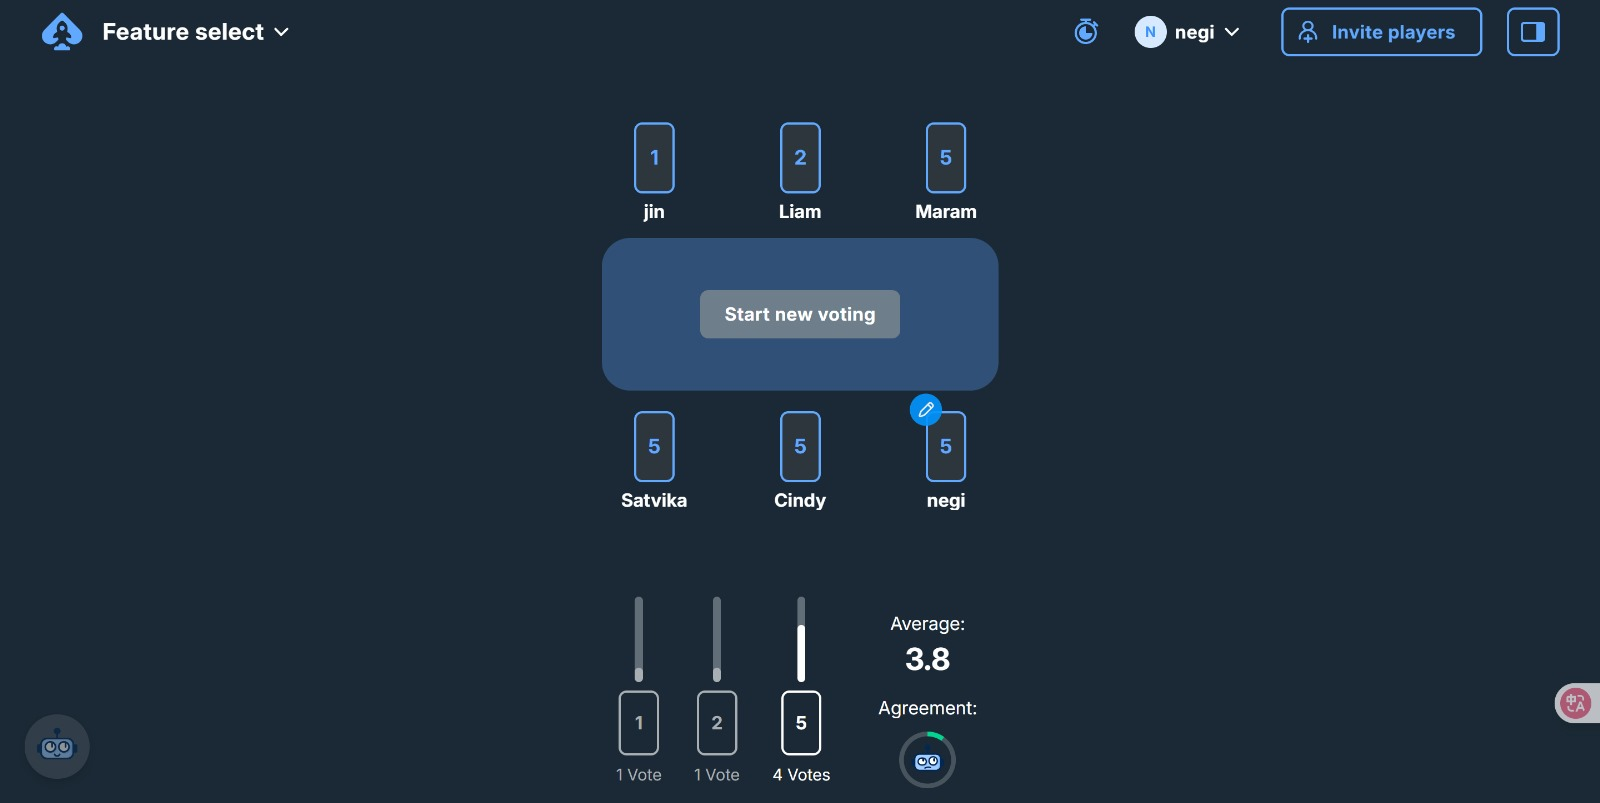
\includegraphics[width=\linewidth]{../../images/planning_poker_low.jpeg}
     \caption{Planning Poker result for the task "doctor records diagnoses," with an average score of 3.8.}
   \end{subfigure}%
   \hfill
   \begin{subfigure}[t]{0.45\textwidth}
     \centering
     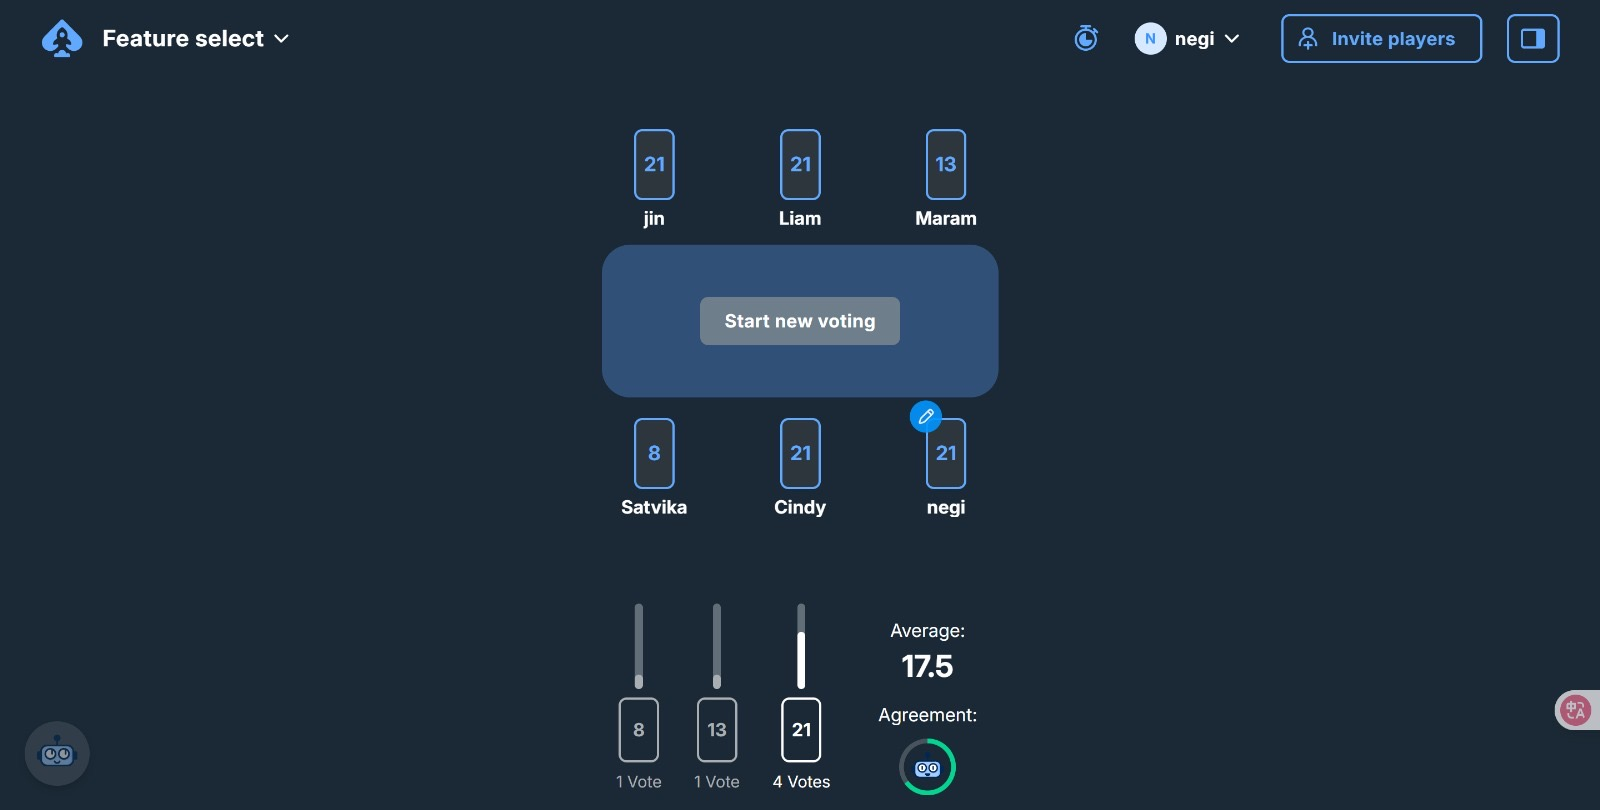
\includegraphics[width=\linewidth]{../../images/planning_poker_high.jpg}
     \caption{Planning Poker result for the task "Health Q\&A," with an average score of 17.5.}
   \end{subfigure}
   \caption{Examples of Planning Poker voting results.}
   \label{fig:planning_poker_examples}
\end{figure}

\paragraph{Bridging Stories and Systems: Workflow Design}\mbox{}\\

After writing the user stories, we started thinking about how these functions could actually connect with each other. For example, if a nurse records the patient’s blood pressure, the doctor should be able to see this data at the next visit. When the doctor checks the medical history and writes the diagnosis, the patient can then see the advice given by the doctor, and so on.

To make these workflows clearer, we drew user flow diagrams in Figma to show the paths of different roles in the system. As shown in Figure~\ref{fig:userflow-registration}, we began with the most basic authentication process, including login, registration, and password reset, so that all users can access the system.

\begin{figure}[H]
   \centering
   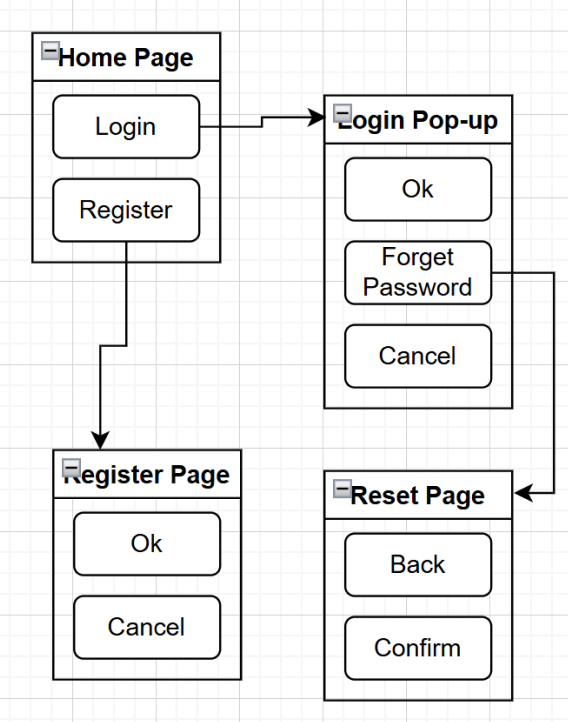
\includegraphics[width=0.4\linewidth]{../../images/userflow_registration.png}
   \caption{User flow diagram for the registration process.}
   \label{fig:userflow-registration}
\end{figure}

Next, we designed the main workflow for the patient role, as shown in Figure~\ref{fig:userflow-whole}. Starting from the dashboard, the patient can use the sidebar to navigate to different pages, including patient intake, patient profile, vital records, and prescriptions. Each page also contains the sidebar and a log-out option, so that the user can switch between functions and log out at any time.
\begin{figure}[H]
   \centering
   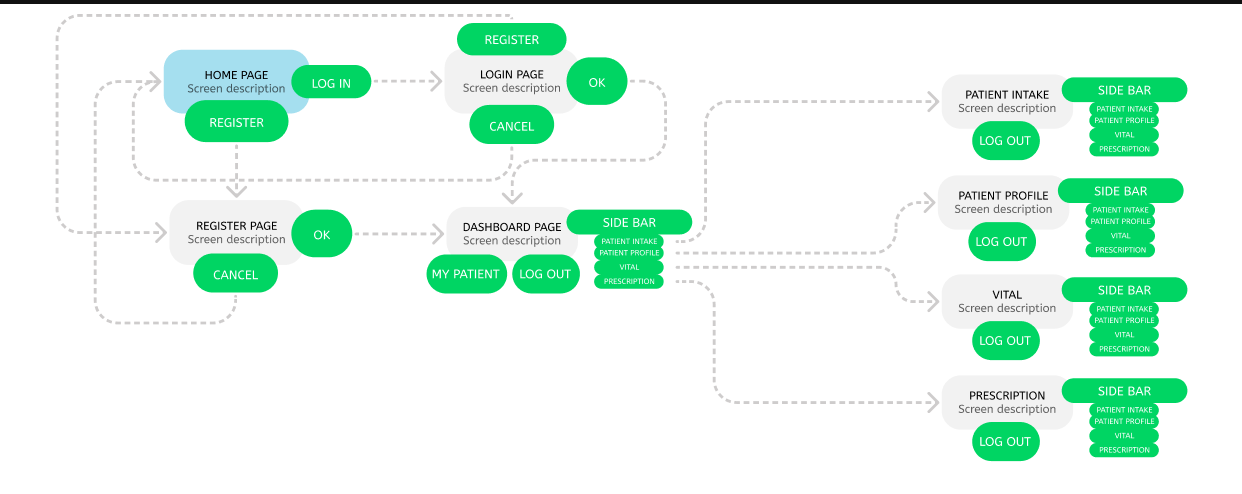
\includegraphics[width=1.1\linewidth]{../../images/userflow_whole.png}
   \caption{Overall user flow diagram of the system.}
   \label{fig:userflow-whole}
\end{figure}


For the function design on each role side, we followed how real hospitals usually work.
Patients can only see their own records and cannot see other people’s information.
For now, nurses can only enter vital signs.
Doctors have the most functions: they can view the full medical history and write diagnoses,
but they cannot change the patient’s basic information.
This setup is similar to how real hospitals operate. 

One difference from real hospitals is that we also considered the remote consultation process.
After the patient makes an appointment, they can first see the doctor from home.
If the doctor thinks it is needed, the patient will then go to a clinic to measure vital signs
or go to the hospital for further treatment.
This can reduce unnecessary visits, and at the same time, still make sure we do not miss any patients who really need care.

The user flow diagrams we drew in Figma helped us make sure each function connects smoothly,
and they also gave the frontend team a clear reference for page navigation.
At this stage, we clarified the logic of the hospital side.
For example, the user must log in before entering the dashboard,
and from the dashboard, they can directly or indirectly access all the designed pages.
These two basic user flow diagrams gave us a clear direction when we started designing the webpages.

\paragraph{Visualizing Functionality: Prototyping with Figma}\mbox{}\\
After we completed the workflow diagram, we used it as the foundation to divide tasks among team members. Each member is responsible for designing specific pages for different parts of the website while working all within a single file, shown as Figure~\ref{fig:3-2-2-DS-figma-f1}, simplified cross-reviewing and allowed for seamless handoffs instead of manually sending assets or screenshots . Next, we will introduce our layout design.
\begin{figure}[H]
  \centering
  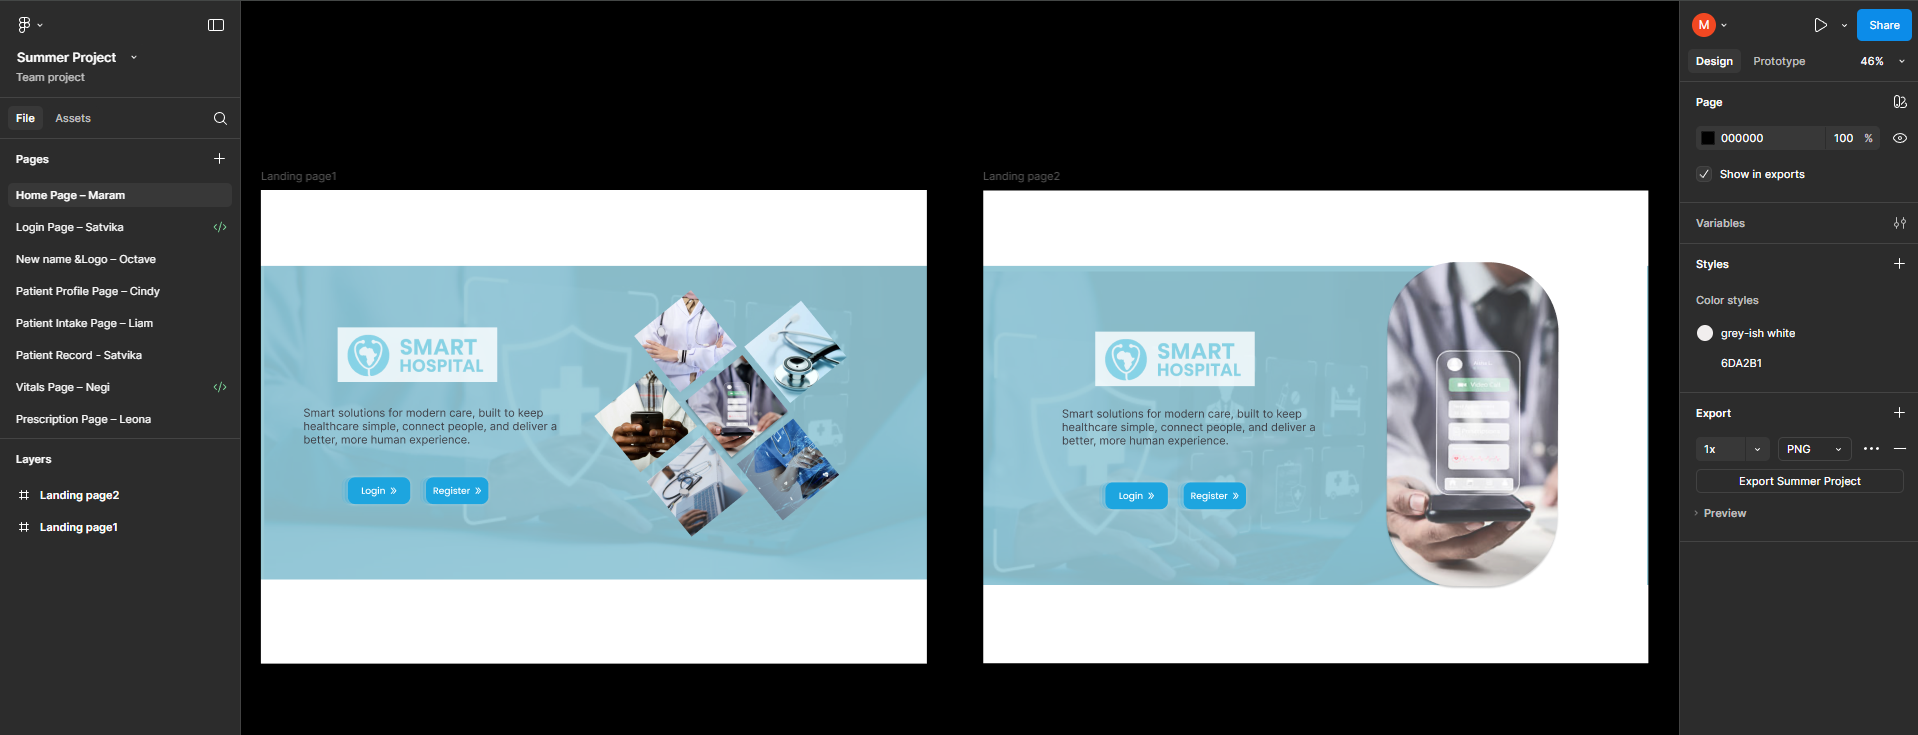
\includegraphics[width=0.8\linewidth]{images03/3-2-2-figure1.png}
  \caption{Shared Figma file displaying landing pages by Maram.}
  \label{fig:3-2-2-DS-figma-f1}
\end{figure}

The primary goal of our layout is to ensure intuitive user interaction. For example when doctors are diagnosing a patient, they typically start by reviewing the patient’s profile to gain a comprehensive understanding of the patient’s condition. This information is displayed on the “Patient Profile” page. At the same time, doctors may need access to the patient’s visits history, so we design a clear and concise list that displays the date of each visit, a brief summary of the diagnosis, and the attending physician. If more detailed information is needed, doctors can click the “view” button to open a pop-up window showing the full report. Another example is during the diagnosis process–doctors may want to take temporary notes before writing the final prescription or summary. To support this, we included a text area on the “Clinical Notes” page where doctors can write their notes down. These features are all designed to enhance the experience for medical professionals interacting with our platform.

Color selection plays a vital role in website design. In our project, we choose a range of blue tones as the primary color scheme, as blue often represents inclusiveness and trust. To make the overall atmosphere feel more approachable and friendly, we incorporate some earthy tones into the blue. Meanwhile, white and gray is used for  elements like buttons and text areas to create a clean and orderly appearance. Through these color combinations, we aim to convey a sense of stability and warmth to our users. The overall visual design reflects the spirit of our platform, to serve as a strong and trustworthy support for users of all ages, genders, physical conditions and cultural background.

We continually review each other’s work using the comment feature which is one of the most useful features we employed, to ensure real-time feedback and update.Throughout the development of each screen, we actively left comments for one another, either suggesting improvements or pointing out issues to be addressed. These comments were visible directly on the relevant design elements, helping us avoid miscommunication and track suggested changes efficiently.

We often initiated discussions either directly within Figma or first during our meetings, and then documented the agreed-upon feedback using the comment feature to ensure accountability. This helped prevent any feedback from being forgotten and gave each designer a clear to-do list for updates. For instance, comments could be left directly on the design (Figure~\ref{fig:figma-comments-example-direct}) or used to track resolved issues after a meeting (Figure~\ref{fig:figma-comments-example-direct-afmeetings}).
\begin{figure}[htbp]
  \centering
  \captionsetup[subfigure]{labelformat=simple, labelsep=space, justification=centering}
  \renewcommand{\thesubfigure}{(\alph{subfigure})}
  \begin{subfigure}[t]{0.48\linewidth}
    \centering
    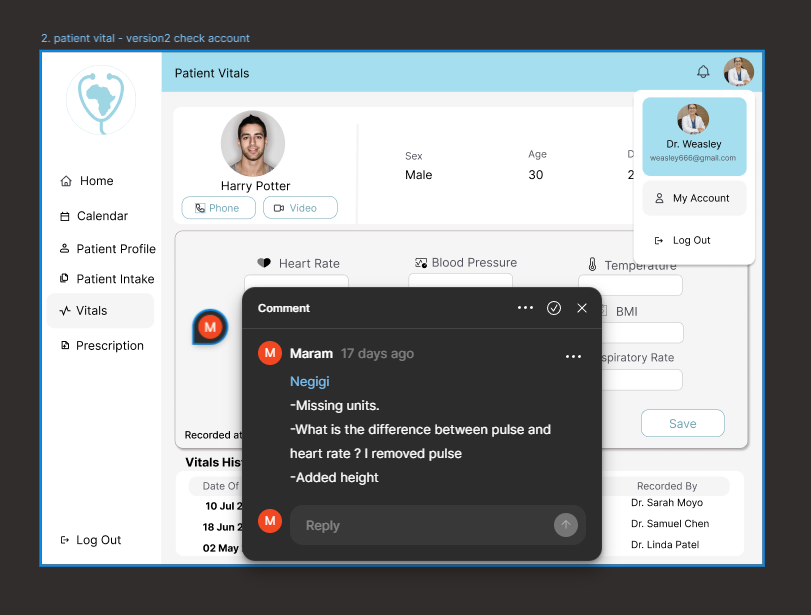
\includegraphics[height=6cm]{images03/3-2-2-figure2.png}
    \caption{Providing feedback via comments.}
    \label{fig:figma-comments-example-direct}
  \end{subfigure}\hfill
  \begin{subfigure}[t]{0.48\linewidth}
    \centering
    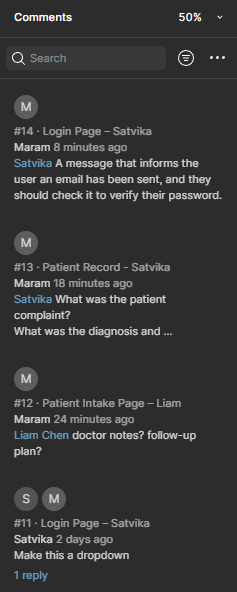
\includegraphics[height=6cm]{images03/3-2-2-figure3.png}
    \caption{Tracking and resolving design feedback.}
    \label{fig:figma-comments-example-direct-afmeetings}
  \end{subfigure}
  \caption{Using Figma's comment feature for collaborative design reviews.}
  \label{fig:figma-collaboration-comments}
\end{figure}

To evaluate whether the designs meet our requirements, we test various user scenarios using Figma’s prototyping feature to link different steps and assess the overall flow. Also, we shared links to Figma with our academic supervisor during our weekly review sessions so that they could view the prototype live. During these review sessions, we made use of the "Follow" feature so that we were all concentrated on the same element of the design so that it was simpler for the supervisor to provide targeted, contextual feedback on specific areas.

This direct communication also allowed us to quickly clarify and allowed us to reduce uncertainty about comments such as "this needs to be more visible" or "consider redesigning this layout."

Moreover, Figma’s version history feature allowed us to continuously improve our design by reflecting on what worked and what didn’t. Although we didn’t manually take snapshots, Figma automatically saved our progress, which made it easy to revisit previous versions at any point. This proved especially helpful when comparing earlier designs with more refined iterations, as it allowed us to clearly see what had improved and what needed further adjustment.

A great example of this is the evolution of the Vitals page, which went through at least six major visual and functional changes, shown in Figure~\ref{fig:vitals-evolution}. In the earliest version, the layout lacked structure, had no sidebar for navigation, and missed key interactive elements such as the "Save Vitals" button, as shown in Figure~\ref{fig:vitals-v1}. As feedback was gathered through team discussions and supervisor input, we iteratively refined the page. By the sixth version (Figure~\ref{fig:vitals-v6}), the design included:

\begin{itemize}
    \item An aligned, visually consistent layout that matches the rest of the system.
    \item A patient card was added at the top to remind clinicians whose record they were updating.
    \item A "Save Vitals" button to improve usability.
    \item A vitals history table, allowing easy access to previously recorded data.
\end{itemize}

% The figure is split into two parts to allow a page break.
\begin{figure}[H] % Part 1 of the figure
  \centering
  \captionsetup[subfigure]{labelformat=simple, labelsep=space, justification=centering}
  \renewcommand{\thesubfigure}{(\alph{subfigure})}
  \begin{subfigure}[t]{0.48\linewidth}
    \centering
    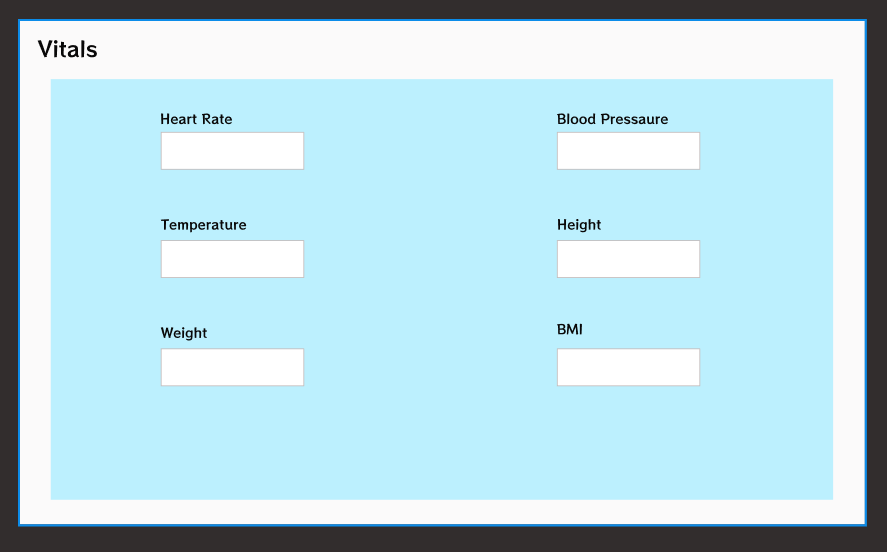
\includegraphics[height=6cm]{images03/3-2-2-figure4a.png}
    \caption{}
    \label{fig:vitals-v1}
  \end{subfigure}\hfill
  \begin{subfigure}[t]{0.48\linewidth}
    \centering
    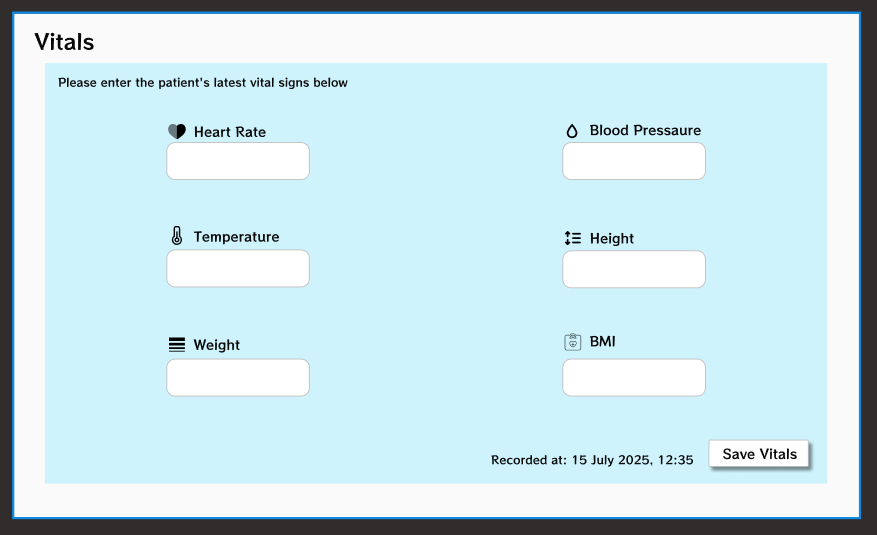
\includegraphics[height=6cm]{images03/3-2-2-figure4b.png}
    \caption{}
    \label{fig:vitals-v2}
  \end{subfigure}
\end{figure}
\begin{figure}[H]\ContinuedFloat
  \par\smallskip
  \begin{subfigure}[t]{0.48\linewidth}
    \centering
    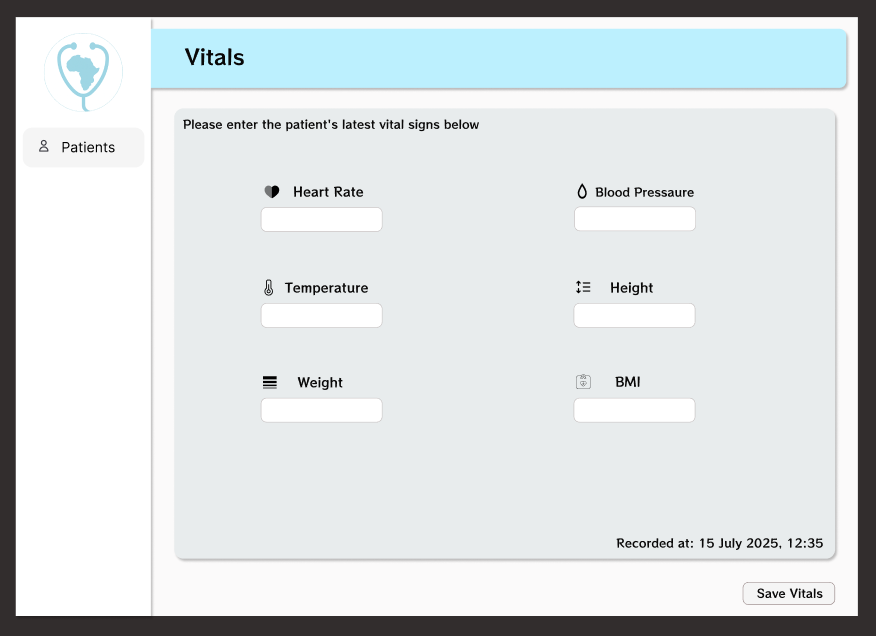
\includegraphics[height=6cm]{images03/3-2-2-figure4c.png}
    \caption{}
    \label{fig:vitals-v3}
  \end{subfigure}\hfill
  \begin{subfigure}[t]{0.48\linewidth}
    \centering
    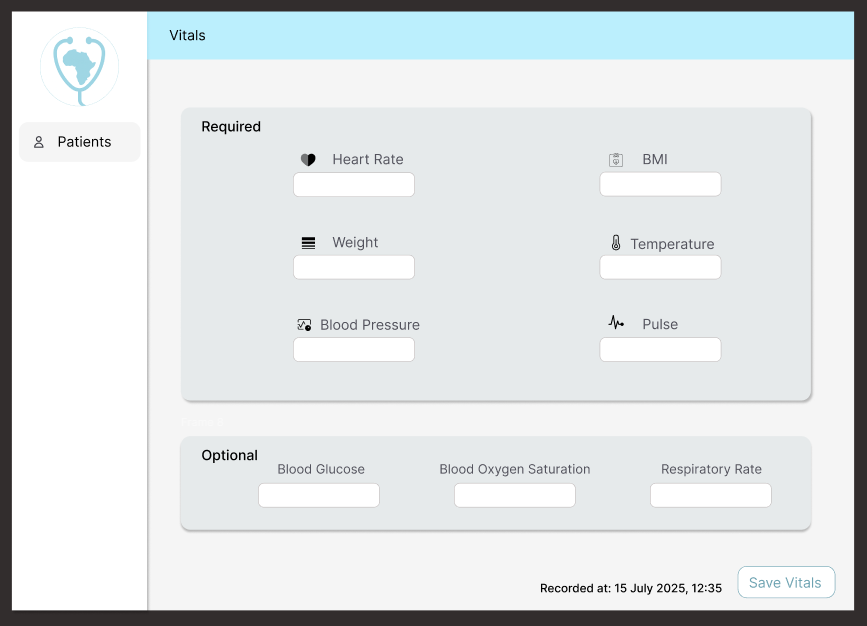
\includegraphics[height=6cm]{images03/3-2-2-figure4d.png}
    \caption{}
    \label{fig:vitals-v4}
  \end{subfigure}
\end{figure}
\begin{figure}[H]\ContinuedFloat % Part 2 of the figure
  \centering
  \begin{subfigure}[t]{0.48\linewidth}
    \centering
    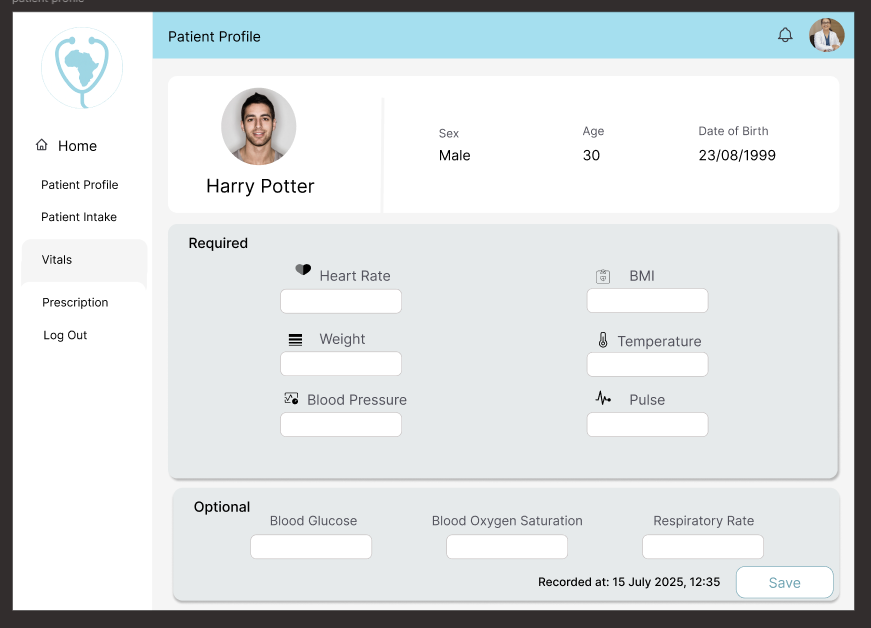
\includegraphics[height=6cm]{images03/3-2-2-figure4e.png}
    \captionsetup{justification=centering}
    \caption{}
    \label{fig:vitals-v5}
  \end{subfigure}\hfill
  \begin{subfigure}[t]{0.48\linewidth}
    \centering
    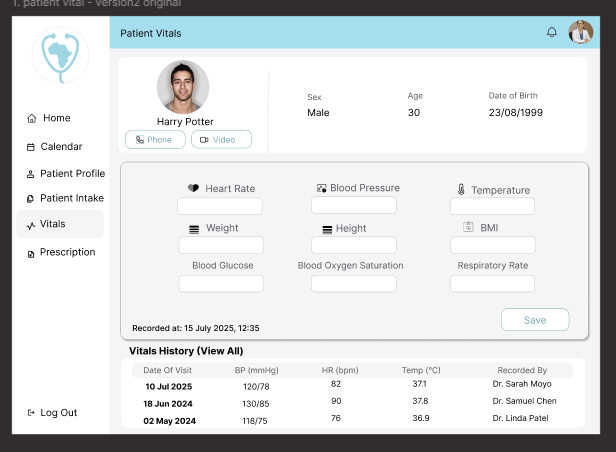
\includegraphics[height=6cm]{images03/3-2-2-figure4f.png}
    \captionsetup{justification=centering}
    \caption{}
    \label{fig:vitals-v6}
  \end{subfigure}
  %\captionsetup{justification=centering}
  \caption{The iterative design process of the Vitals page, showing its evolution through six key versions. (a) Basic layout without a sidebar or patient card. (b) Introduction of a navigation sidebar. (c) Adding a patient information card at the top. (d) Refining the layout and adding a history table. (e) Improving visual consistency and button placement. (f) Final design with all key components integrated.}
  \label{fig:vitals-evolution}
\end{figure}

These changes not only enhanced the interface visually, but also made the page much more usable in a real clinical workflow. Since healthcare professionals often move quickly between patient records, having the patient card consistently displayed at the top of all patient-specific pages helps reduce confusion, reminding them of whose data they are viewing or editing.

We made multiple adjustments to several pages based on weekly feedback from our supervisor and internal team reviews. This ensured a more user-friendly and functional design across the platform.

One of the most significant design iterations in our project involved the Prescription Page. During a weekly meeting with our supervisor, we received feedback that the initial layout appeared empty and lacked the essential clinical details typically expected in a real-world healthcare system. Based on this feedback, we conducted research into existing healthcare system standards to understand what prescription interfaces should contain, with a particular focus on NHS guidelines and clinical UX principles.

% NOTE: Please replace 'rcp_med_standards' and 'nhs_design_system' with the correct keys from your thesisbiblio.bib file.
We referred to the \emph{Medication and Allergy Standards for structured records}, published by the Royal College of Physicians in collaboration with the Health and Social Care Information Centre (HSCIC) in 2013. These standards recommend that digital prescriptions should include key information such as medication name, dosage, frequency, route, duration, and notes, all of which are fields we implemented in our updated interface~\cite{rcp_med_standards}.

In terms of user interface design, we followed the NHS Design System’s guidance on card components, which recommends grouping related form fields into visually distinct blocks. This improves usability and reduces cognitive load by allowing clinicians to focus on one section at a time. Inspired by this, we introduced structured “Medication Cards” in our interface, each containing fields for medication name, dosage (e.g., 500mg), frequency (e.g., twice a day), route (e.g., oral or IV), duration (e.g., for 7 days), and clinical notes (e.g., take before meals). We also added a dropdown for selecting saved medication records, improving both usability and completeness of the page~\cite{nhs_design_system}.

These changes transformed the original sparse interface into a more complete, user-friendly, and clinically appropriate design. They also align our application with industry standards for both content structure and interface design, as shown in Figure~{\ref{fig:prescription-evolution}}.

\begin{figure}[htbp]
  \centering
  \captionsetup[subfigure]{labelformat=simple, labelsep=space, justification=centering}
  \renewcommand{\thesubfigure}{(\alph{subfigure})}
  \begin{subfigure}[t]{0.48\linewidth}
    \centering
    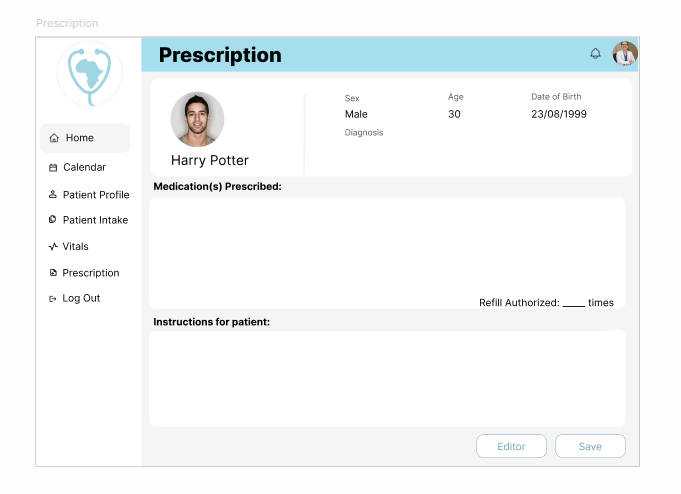
\includegraphics[height=6cm]{images03/3-2-2-figure5a.png}
    \caption{}
    \label{fig:prescription-before}
  \end{subfigure}\hfill
  \begin{subfigure}[t]{0.48\linewidth}
    \centering
    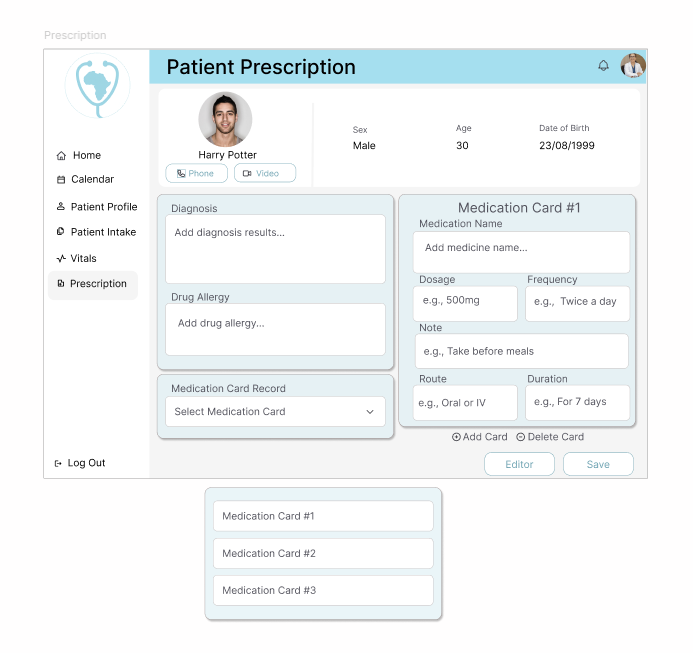
\includegraphics[height=6cm]{images03/3-2-2-figure5b.png}
    \caption{}
    \label{fig:prescription-after}
  \end{subfigure}
  \caption{Comparison of the Prescription Page before and after design iteration based on supervisor feedback. (a)Initial design of the Prescription Page. (b)Redesigned page with structured ``Medication Cards'' and comprehensive fields, following NHS guidelines.}
  \label{fig:prescription-evolution}
\end{figure}

Similarly, during one of our internal design review meetings, we identified a gap in the Patient Profile Page. Initially, the Patient Profile Page featured the doctor’s profile picture, but it lacked interactivity. In a later iteration, we enhanced the design by implementing a functional popup menu. This allowed doctors to either access their account settings or securely log out, improving both usability and navigation consistency, as shown in Figure~{\ref{fig:profile-menu-evolution}}. These feedback-driven design iterations not only improved usability but also aligned the interface with real-world clinical workflows and recognized healthcare UI standards.

\begin{figure}[H]
  \centering
  \captionsetup[subfigure]{labelformat=simple, labelsep=space, justification=centering}
  \renewcommand{\thesubfigure}{(\alph{subfigure})}
  \begin{subfigure}[t]{0.48\linewidth}
    \centering
    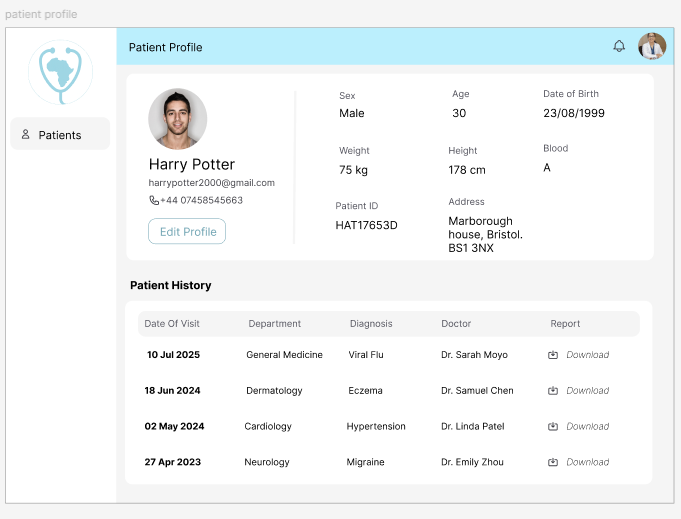
\includegraphics[height=6cm]{images03/3-2-2-figure6a.png}
    \caption{}
    \label{fig:profile-menu-before}
  \end{subfigure}\hfill
  \begin{subfigure}[t]{0.48\linewidth}
    \centering
    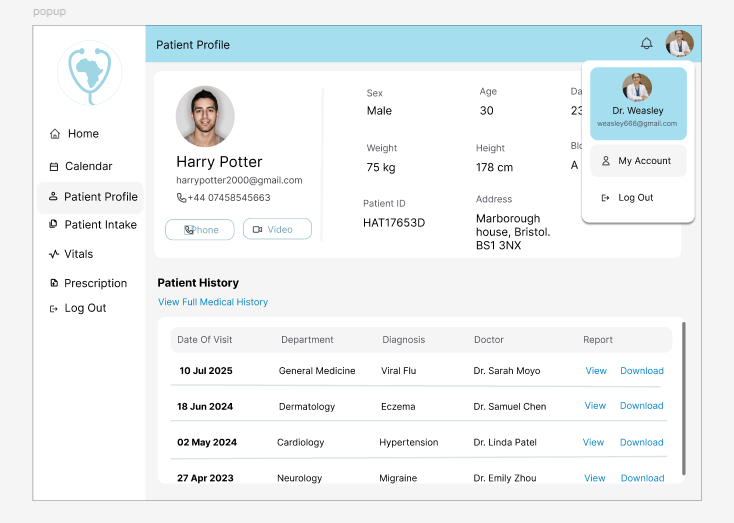
\includegraphics[height=6cm]{images03/3-2-2-figure6b.png}
    \caption{}
    \label{fig:profile-menu-after}
  \end{subfigure}
  \caption{Evolution of the doctor's profile menu on the Patient Profile Page. (a)Initial design with a static, non-interactive doctor profile picture. (b)Enhanced design with a functional popup menu for account settings and logout.}
  \label{fig:profile-menu-evolution}
\end{figure}



\paragraph{Front-end Implementation}\mbox{}\\

In the front-end implementation section, we illustrate the process of how we created, organised, and tested our front-end code. We divide this process into 5 stages. First, we describe how we structured and developed the codebase. Then, we explain how we integrate shared layouts using Thymeleaf to improve consistency and maintainability across pages. Next, we explain how different pages are connected to form a smooth user flow. We also discuss the steps we took to test each function to ensure the website behaves as intended. Finally, we reflect on the main challenges we encountered during the front-end development and how we addressed them. These topics are covered in following subsections: Code Structure and Component Organisation, Integrating Shared Layouts with Thymeleaf, Page Navigation and User Flow, User Flow and Functional Testing, and Challenges Encountered During Frontend Development, respectively.
\paragraph{Code Structure and Component Organisation}\mbox{}\\
In this section, we describe how we constructed the front-end codebase. As mentioned earlier, each member was responsible for designing different parts of the website in Figma. We continued the pattern during implementation–each member developed their assigned parts using HTML and CSS, focusing on accurately reproducing the layout and visual style from our Figma design.

At this stage, our goal is to replicate the layout and visual style of our Figma design. Most interactive elements, such as buttons, pop-up windows, and form submissions, have not yet been functionalized. We have also not yet integrated a shared layout system using Thymeleaf. These shared elements are currently duplicated across individual pages, and we plan to organize them in the next development stage to improve maintainability and consistency.

\paragraph{Integrating Shared Layouts with Thymeleaf}\mbox{}\\
After developing all the pages, we noticed that many structural elements–such as headers, sidebars, and forms–were repeated across different pages. To reduce redundancy and to make the Smart Hospital UI consistent and maintainable, we wrapped repeated interface components (sidebar, top navigation, and patient header) into reusable Thymeleaf fragments and consumed them across pages with th:replace. As shown in Figure~\ref{fig:3-2-2-vital-history-page}, the vitalsHistoryPage.html file defines an empty container, CSS links, outer grid, and main content area, while common UI components are injected at render time from layouts/sharedLayout.html.

\begin{figure}[H]
  \centering
  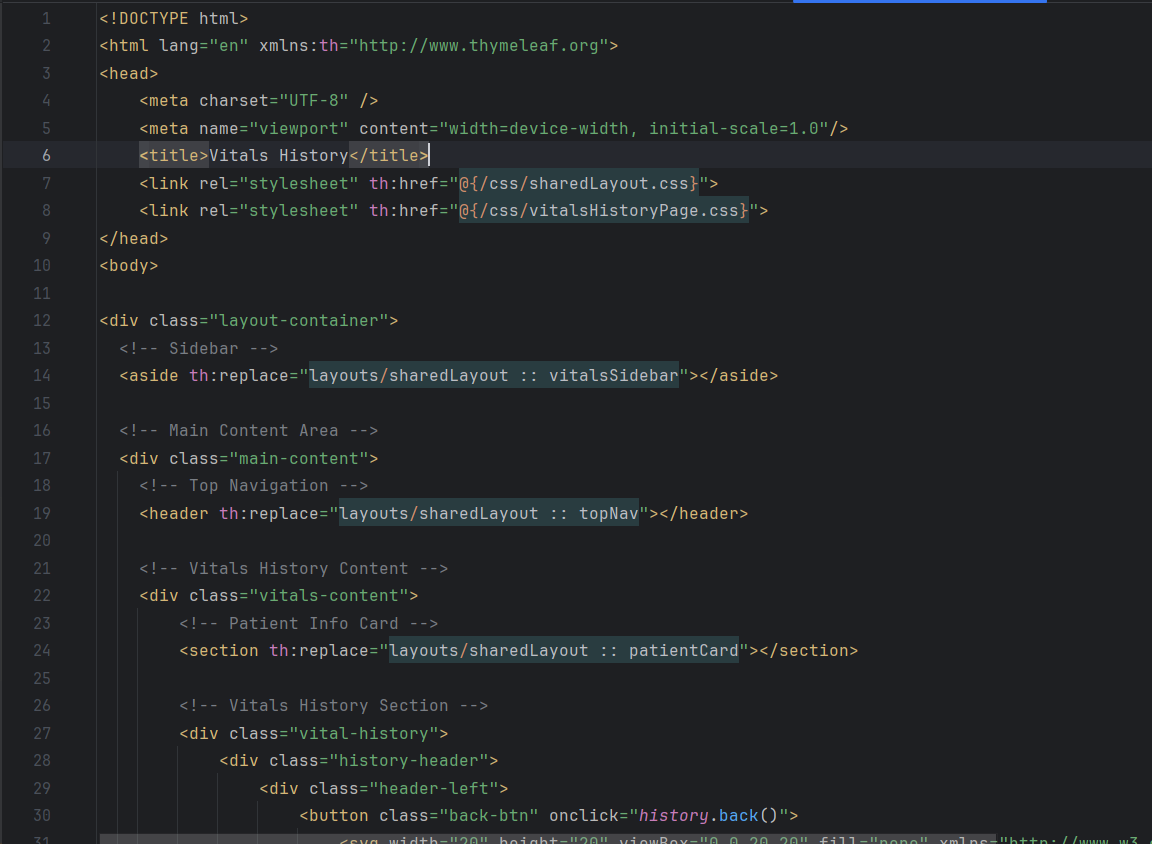
\includegraphics[width=0.8\linewidth]{images03/3-2-2-vitalHS.png}
  \caption{vitalsHistoryPage.html consuming shared fragments (vitalsSidebar, topNav, patientCard) via th:replace.}
  \label{fig:3-2-2-vital-history-page}
\end{figure}

For example, the Vitals page loads the active vitalsSidebar fragment (highlighting the Vitals tab), the topNav fragment (with dynamic pageTitle provided via the model), and a patientCard fragment (so clinicians can always see the patient context at the top of patient-specific pages). This server-side composition makes our design system dry, updating the sidebar icon set or the patient header once applied everywhere without touching individual pages. Figure~\ref{fig:3-2-2-sharedLayout} illustrates part of the sharedLayout.html file, displaying the sidebar fragment and its logo and most crucial navigation links.

\begin{figure}[H]
  \centering
  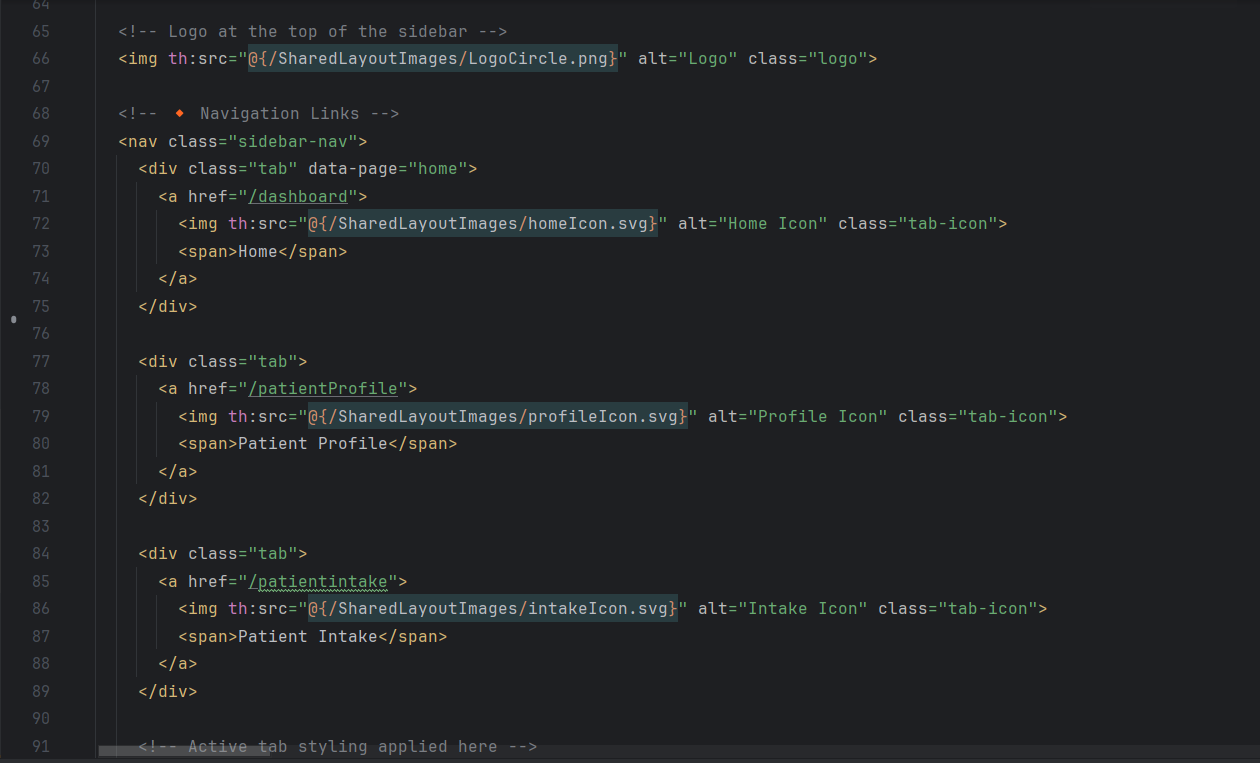
\includegraphics[width=0.8\linewidth]{images03/3-2-2-sharedLayout.png}
  \caption{Snippet from sharedLayout.html showing the sidebar fragment, including the logo at the top and navigation links.}
  \label{fig:3-2-2-sharedLayout}
\end{figure}

We also separated shared and page-specific styling concerns to avoid cascade conflicts. Fragment-level styles for global pages live in \verb|sharedLayout.css| and are loaded ahead of each page's own stylesheet (e.g., \verb|vitalsHistoryPage.css|). Fragments leverage Thymeleaf's URL syntax (e.g., \verb|th:src="@{/SharedLayoutImages/}"|) to refer to assets so paths get resolved properly no matter the environment. Where a page needs alternative "active" navigation, we provide a purpose-specific fragment (e.g., \verb|sidebar| vs. \verb|vitalsSidebar|) to facilitate correct tab state without hardcoded per-page logic. This approach assisted in achieving consistency (the same chrome everywhere), maintainability (one change affects all pages), and clarity. As shown in Figure~\ref{fig:3-2-2-renderLayout}, clinicians always have navigation context and the patient card visible when navigating between modules.

\begin{figure}[H]
  \centering
  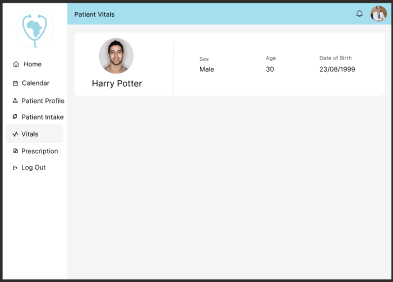
\includegraphics[width=0.8\linewidth]{images03/3-2-2-renderLayout.png}
  \caption{Rendered UI in the browser showing the shared sidebar, patient card, and top navigation in the Vitals module.}
  \label{fig:3-2-2-renderLayout}
\end{figure}

\paragraph{Page Navigation and User Flow}\mbox{}\\
In this stage, we began to functionalize interactive elements such as buttons, hyperlinks to ensure the website provides a smooth and intuitive experience. The overall user flow had already been defined in our early-stage Figma design, a clear user flow that reflects typical interactions between patients and doctors in our early-stage Figma design, reflecting typical interactions between patients and doctors. Each page was connected according to the logical steps users would take when navigating through the platform. For example, clicking the “Register” button on the homepage directs users to the registration form, and buttons on the “Dashboard” page are linked to corresponding pages. These workflows were clearly visualized in our Figma prototype. The main goal of this stage is to ensure that all the interactive elements function as the origin design. In the next stage, we plan to test the whole website work appropriately and collect the disadvantages that can be improved.
\paragraph{User Flow and Functional Testing}\mbox{}\\

\paragraph{Challenges Encountered During Frontend Development}\mbox{}\\
One of the biggest challenges encountered while performing frontend development was how to break down the Figma-based design system into Thymeleaf templates. Even though the Figma designs created a solid visual reference for layout, typography, and spacing between elements, the server-side rendering approach of Thymeleaf required the interface to be split into smaller, more manageable parts. It introduced additional difficulty in the process of converting pixel-perfect designs into coherent HTML templates with alignment, responsiveness, and style consistency preserved. Visual parity usually needed to be delivered by iterative adjustments of the HTML structure as well as accompanying CSS.

An analogous problem involved the handling of shared styles and bits within the multi-page Thymeleaf application. Shared interface pieces, the sidebar navigation, header, and footer, were included as reusable fragments to foster consistency and reduce redundancy. With this came, however, the risk of side effects: a modification of a shared fragment would likely disrupt the styling or layout of multiple pages. To tackle this, the development team implemented a formalized update process, such as fragment-specific testing and peer review prior to merge of changes. This procedure ensured global component updates maintained visual correctness without causing regressions in other parts of the system.


\chapter{Back-end Design and Implementations}
\label{sec:sec03}

\section{Setup and Tools}
\label{subsubsec:dbsetup}
\paragraph{Programming Language}\mbox{}
\paragraph{Database}\mbox{}

\section{Database Design}
\label{subsubsec:Database Design}
% File: chap03-03-02.tex
% Author:
% Description:
% 3.3 Back-end Design & Implementation
%  3.3.2 Database Design
%     Entity Relationship Design
%     Database Schema Implementation
%     Data Security and Privacy Considerations
%

After we finished the detailed discussion of each page’s user flow, we moved on to database design. Our first task was to clarify what kinds of data the system must store, and map them to a clear set of entities and relationships. We first created a rough data model on dbdiagram.io \citep{dbmldocs} as a quick way to communicate and iterate. During modelling, we noticed several issues in button navigation and page flow. To avoid a mismatch between frontend and backend, we worked in parallel—“draw the diagram and verify the flow at the same time”—and actively met with teammates to unify the detailed flows and the data to read/write. After that, for every system button or operation, we traced back the required primary/foreign keys and necessary column types, and then integrated all of these needs into the final data model.

% 確保有載入:\usepackage{graphicx}



The system’s full relationship structure is shown with crow’s-foot notation \citep{crowsfoot}. We implemented the revised schema in MySQL and used DBeaver’s reverse engineering \citep{dbeaverERD} to automatically generate the ERD from the live database. All ERDs in the final report were exported from DBeaver to ensure the diagrams match the actual tables, as shown in Figure~\ref{fig:final_erd}.

\begin{figure}[!htbp]
  \centering
  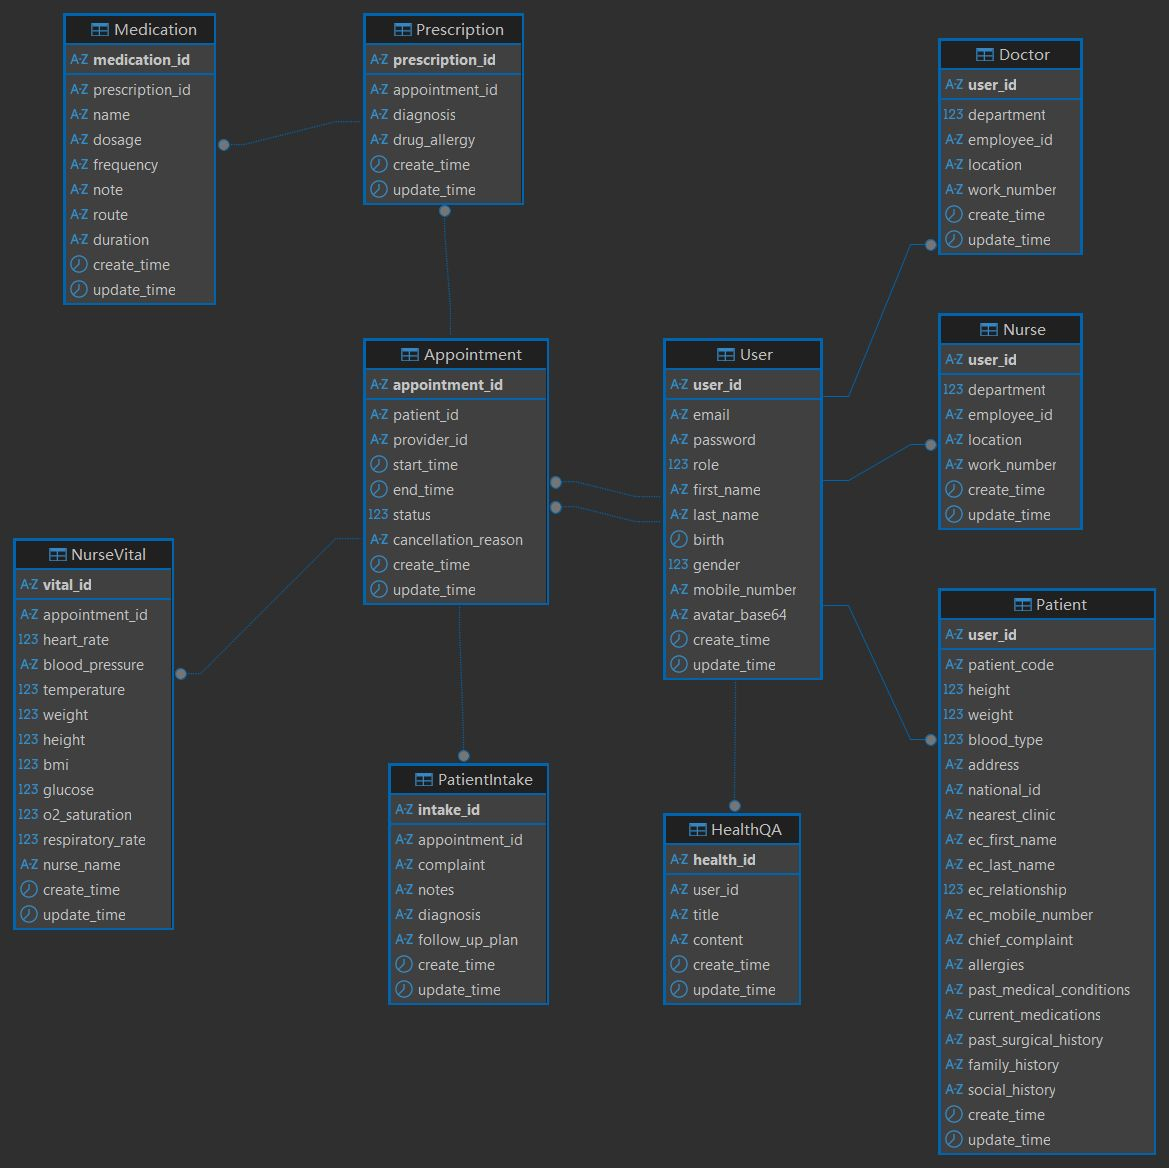
\includegraphics[width=\linewidth]{../../images/ERD.jpeg}
  \caption{Final ERD (reverse-generated from MySQL via DBeaver \protect\citep{dbeaverERD}).}
  \label{fig:final_erd}
\end{figure}
\FloatBarrier

From the figure, you can see an appointment-centred, single-visit data flow. \texttt{NurseVital} and \texttt{PatientIntake} (renamed on the frontend as \textit{Clinical Note}) correspond to nurse and doctor records. \texttt{Prescription}, together with multiple \texttt{Medication} rows, describes the treatment plan. For the HealthQA interaction, although we did not implement it due to time limits, we designed the tables so the system is ready for future work. We use a unique index on \texttt{User.email}, a composite index on \texttt{Appointment(patient\_id, provider\_id, start\_time)}, and indexes on all major foreign keys. 

Overall, this data model supports the core operations in our user flows (creating/cancelling appointments, recording vitals, filling consultation summaries, issuing prescriptions, and viewing medical history) while leaving space for extensions like report files and the Health Q\&A feature, keeping the Smart Hospital system consistent and maintainable.


\section{Testing}
\label{subsubsec:dbtesting}
%% File: chap03-03-02.tex
% Author:
% Description:
% 3.3 Back-end Design & Implementation
%  3.3.2 Database Design
%     Entity Relationship Design
%     Database Schema Implementation
%     Data Security and Privacy Considerations
%

After we finished the detailed discussion of each page’s user flow, we moved on to database design. Our first task was to clarify what kinds of data the system must store, and map them to a clear set of entities and relationships. We first created a rough data model on dbdiagram.io \citep{dbmldocs} as a quick way to communicate and iterate. During modelling, we noticed several issues in button navigation and page flow. To avoid a mismatch between frontend and backend, we worked in parallel—“draw the diagram and verify the flow at the same time”—and actively met with teammates to unify the detailed flows and the data to read/write. After that, for every system button or operation, we traced back the required primary/foreign keys and necessary column types, and then integrated all of these needs into the final data model.

% 確保有載入:\usepackage{graphicx}



The system’s full relationship structure is shown with crow’s-foot notation \citep{crowsfoot}. We implemented the revised schema in MySQL and used DBeaver’s reverse engineering \citep{dbeaverERD} to automatically generate the ERD from the live database. All ERDs in the final report were exported from DBeaver to ensure the diagrams match the actual tables, as shown in Figure~\ref{fig:final_erd}.

\begin{figure}[!htbp]
  \centering
  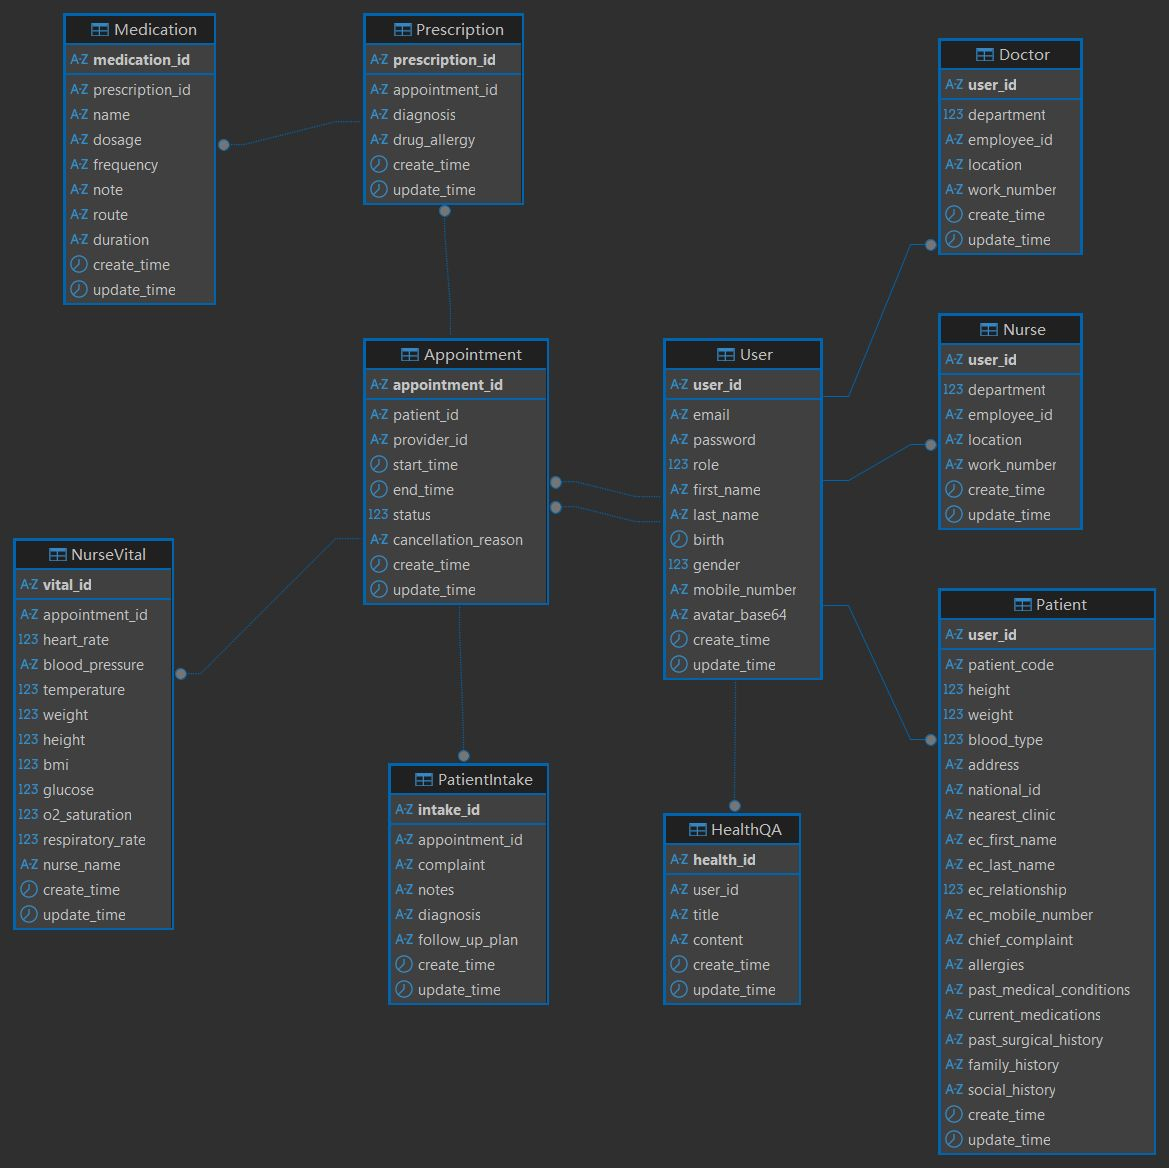
\includegraphics[width=\linewidth]{../../images/ERD.jpeg}
  \caption{Final ERD (reverse-generated from MySQL via DBeaver \protect\citep{dbeaverERD}).}
  \label{fig:final_erd}
\end{figure}
\FloatBarrier

From the figure, you can see an appointment-centred, single-visit data flow. \texttt{NurseVital} and \texttt{PatientIntake} (renamed on the frontend as \textit{Clinical Note}) correspond to nurse and doctor records. \texttt{Prescription}, together with multiple \texttt{Medication} rows, describes the treatment plan. For the HealthQA interaction, although we did not implement it due to time limits, we designed the tables so the system is ready for future work. We use a unique index on \texttt{User.email}, a composite index on \texttt{Appointment(patient\_id, provider\_id, start\_time)}, and indexes on all major foreign keys. 

Overall, this data model supports the core operations in our user flows (creating/cancelling appointments, recording vitals, filling consultation summaries, issuing prescriptions, and viewing medical history) while leaving space for extensions like report files and the Health Q\&A feature, keeping the Smart Hospital system consistent and maintainable.


\section{API}
\label{subsubsec:dbdesign}
%
% File: chap03-03-03.tex
% Author: PINRU & LEONA
% Description:
% 3.3 Back-end Design and Implementations
%  3.3.3 API
%     Design
%     Implementation
%

\paragraph{Design}\mbox{}\\

In our virtual hospital website, the API works as a bridge between the frontend and the backend database. When we designed it, we mainly consider two things. One is the database rules, for example, username must be unique, and inputs should be checked. The second is the frontend use, like doctor or patient register and login, booking appointments, or searching hospital information. Since the request style is quite simple and mostly CRUD, we choose REST style and use Spring MVC.

For page rendering, we use Thymeleaf for server-side rendering. Something like GET /patient/manageAppointments will send back a HTML page with data already put inside. But when it is about actions that need fast response, like cancel appointment or refresh it, the frontend send AJAX to get JSON, for example POST /patient/appointments/cancel/{id} or GET /patient/appointments/refresh. Only part of the page will update, not reload the whole one. This mixed design, SSR for pages and JSON for small actions, makes first loading faster and user feeling smoother, and it is still not so complex.

To keep the API easy to use, we try to follow same rules for endpoint names, HTTP verbs and status code. Like GET is for reading data, POST for create, 200/201 for success, and clear error when validation fails. The controller will check important fields, like if password match or ID card and phone format. In the future, when database and permission are added, authentication and authorization can also be put under same endpoints, so frontend work flow will not be broken.

\clearpage

\paragraph{Implementation}\mbox{}\\

During the implementation, we used Spring Boot 3.5.3 with MyBatis for the database operation, which follows the patterns of a layered architecture \cite{fowler2002}. We are writing the actual API requests based on the API specification instructions.

The majority of the APIs are built similarly. For annotations like @GetMapping, we can set the kind of request type it is, the path it uses, and the response it gives back. The function then safely collects user details and passes them to the service layer methods, for them to handle the request.

Example code is shown below about the patient appointment information:

\begin{figure}[h]
\centering
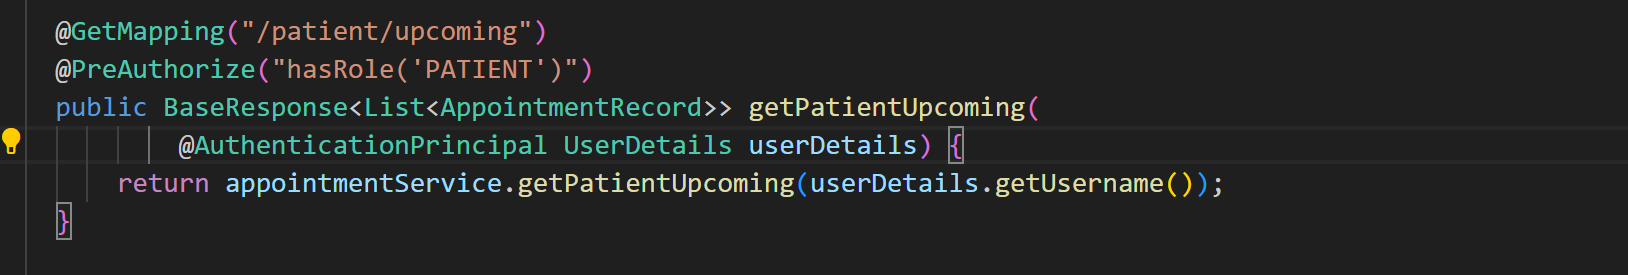
\includegraphics[width=0.8\textwidth]{chapters/chapter03/images03/3-3-1-figure(API-I).png}
\caption{Appointment Controller Implementation Code}
\label{fig:appointment-controller}
\end{figure}

Using @PreAuthorize, this will check the user's permissions and account roles \cite{springsecurity2024}. Using @AuthenticationPrincipal will then extract from Spring Security user information context; this doesn't need to authorise a token through a manual process \cite{johnson2023}.
The appointmentService.getPatientUpcoming() method includes dealing with business logic requests.

For the return type, we use \texttt{BaseResponse<T>}, replacing \texttt{ResponseEntity<ObjectNode>}, which offers the unified JSON structure. This type includes status code, message and data information, when dealing with different request errors, and the format makes it more consistent and clean.

Server methods contain business logic, and we use MyBatis to handle database operations \cite{springsecurity2024}. These functions create, update, delete, or query data through Mapper interfaces. MyBatis offer type-safe database operations and automatic SQL argument binding, compared to traditional JDBC, with fewer sample codes.

Some parts of server methods include more complicated logic, such as appointment scheduling, user personal information management, and health record handling. Those implementation methods not only enhance the optimisation, but also strengthen the system safety through Spring Security, integrate system safety, and provide a clear layer architecture to make the code more unified.


\section{Implementation}
\label{subsubsec:dbimplementation}
\paragraph{Implementation}\mbox{}\\
To implement the database, we converted the conceptual design into a set of SQL queries, available at \url{https://github.com/MaramAbdulaziz1/smart-hospital/tree/main/conf/database.sql}. The entire relational structure is defined in \texttt{database.sql}, ensuring relationships are enforced through primary keys, foreign keys, and appropriate uniqueness constraints. All tables use the InnoDB engine to guarantee transactional consistency and referential integrity. Data types were selected to balance correctness and performance: \texttt{char(36)} for UUIDs, \texttt{datetime} for timestamps, and \texttt{tinyint} for enumerated values (e.g., roles, departments, gender). Default values were set for audit fields such as \texttt{create\_time} and \texttt{update\_time}, and unique constraints prevent duplication in critical identifiers (e.g., emails, employee IDs, patient codes).

\mbox{}\\
Table creation followed the logical dependency graph. The \texttt{User} table was created first as the base referenced by most others. In parallel, \texttt{Doctor}, \texttt{Nurse}, \texttt{Patient}, and \texttt{HealthQA} were created, each referencing \texttt{User} via \texttt{user\_id}. Next, \texttt{Appointment} was defined using \texttt{patient\_id} and \texttt{provider\_id} (a user linked to a clinician). Downstream entities—\texttt{NurseVital}, \texttt{PatientIntake}, and \texttt{Prescription}—reference \texttt{Appointment}, and \texttt{Medication} links to \texttt{Prescription}. This modular decomposition supports scalability and maintainability by keeping domain logic clearly separated across entities. For testing, instead of seeding static SQL fixtures, we inserted mock data through the frontend forms. During development resets, tables were manually cleared and refreshed using DBeaver, our preferred MySQL GUI.


\section{Data Plan}
\label{subsubsec:dbdataplan}
%\input{chap03-03-05.tex}

\section{Authentication and Authorization Function}
\label{sec:auth-auth}
%
% File: chap03-04.tex
% Author: LEONA
% Description:
% 3.4 Authentication and Authorization Function
%  3.4.1 Overview
%  3.4.2 Implementation
%  3.4.3 Password Protection
%  3.4.5 Role-Based Authorization
%  3.4.6 API Summary
%  \clearpage \newpage

\paragraph{3.4.1 Overview}\mbox{}\\

When using this virtual hospital system, users are required to log in first, after which different functions will be displayed based on their roles. Patients can make or cancel appointments. Doctors can check schedules and contact patients. We use SpringSecurity to manage login status and permission control, while retaining a custom login API to match the page flow.

\paragraph{3.4.2 Implementation}\mbox{}\\

Login and logout are inside UserLoginController. For login, the controller use LoginService to check username and password from request. If correct, the service make an Authentication object and put into SecurityContextHolder of Spring Security. Then browser get a session cookie (like JSESSIONID) to keep the user login. For logout, we call SecurityContextLogoutHandler.logout(...) to clear the context and make the session not valid.

\paragraph{3.4.3 Password Protection}\mbox{}\\

We do not keep the real password in the database. Before saving, the password will be hashed, so even if someone see the database, they only find some random string. When user try to login, the system hash the input password again and check if it is same with the stored one. Because medical data is very sensitive, we add this function to protect user account. This way is also a common practice in security and can help to keep the information safe.

\paragraph{3.4.5 Role-Based Authorization}\mbox{}\\

We separate access by URL patterns and roles. Patient features are under /patient/**, and doctor features are under /doctor/**. Spring Security checks the role before the controller executes. If needed, we can add method-level rules such as @PreAuthorize("hasRole('DOCTOR')") for endpoints that are doctor-only. This design keeps the front-end workflow simple while the back-end enforces permissions.



\section{Reservation System Implementation}
\label{sec:reservation-system}
\subsection{System Overview}
\label{subsec:reservation-overview}

According to section 3.4.1, a medical platform can choose traditional and dynamic interactive systems. Traditional form-based technology usually leads to lower user participation and a relatively low completion rate of reservations. Therefore, we chose to implement a system based on RESTful APIs and an instant, dynamic, and interactive updates system at the end.

The whole process of implementation includes three main phases: First, integrate spring-boot-starter-web and spring-boot-starter-security dependencies; Second, build RESTful API endpoints; Lastly, before operating the interface, add AJAX functionality on the frontend to support dynamic interactions with Thymeleaf templates.

\subsection{Appointment Lifecycle and Status Management}
\label{subsec:appointment-lifecycle}

The appointment system implements the whole life cycle, which includes four different statuses. The system supports two types of reservations: doctor clinic and nurse vitals check, and it focuses on different designs' appointment rules and authorisation.

Appointment status cycle:
\begin{itemize}
    \item Upcoming (Initial Status): Patient creates an appointment $\rightarrow$ next step: cancelled
    \item Complete (First Status): Appointment has been completed
    \item Cancelled (Second Status): Appointment could be cancelled by the patients
    \item Expired (Final Status): Appointment has expired due to a past date
\end{itemize}

Status transition rules:
\begin{itemize}
    \item Upcoming status can be transformed to cancelled
    \item Cancelled is the final status, can't be transformed again
    \item Doctors can view their appointments on the dashboard
\end{itemize}

\subsection{Booking Process and Conflict Prevention}
\label{subsec:booking-process}

To ensure appointment accessibility, this system designs a complete conflict prevention mechanism. Before reservation confirmation, the system will implement multiple authorisation checks:

Appointment process:
\begin{itemize}
    \item Patient authorisation check: use @AuthenticationPrincipal to authorise the patient role and login status.
    \item Database constraint validation: prevent double booking through unique key constraints.
    \item uk\_patient\_time: prevents the same patient from booking multiple appointments at the same time
    \item uk\_provider\_time: prevents the same provider from having multiple appointments at the same time
\end{itemize}

The code below showcases the conflict observation appointment flows:

\begin{lstlisting}[language=Java, caption=Appointment Booking Implementation]
@PostMapping("/book")
@PreAuthorize("hasRole('PATIENT')")
public BaseResponse<String> bookAppointment(
    @AuthenticationPrincipal UserDetails userDetails,
    @RequestBody AppointmentBook appointmentBook) {
    return appointmentService.book(userDetails.getUsername(), appointmentBook);
}
\end{lstlisting}

Mapping MyBatis SQL insert is below:

\begin{lstlisting}[language=SQL, caption=Appointment Insert Query]
<insert id="insertAppointment">
    INSERT INTO Appointment
    (appointment\_id, patient\_id, provider\_id, `date`, appoint\_time, status)
    VALUES
    (uuid(), \#{patientId}, \#{providerId}, \#{date}, \#{appointTime}, \#{status})
</insert>
\end{lstlisting}

\subsection{Cancellation Function}
\label{subsec:cancellation-function}

The cancellation system allows a patient to cancel an appointment after authorisation, and then the system updates the appointment status to cancelled.

Cancellation flow:
\begin{itemize}
    \item Authorisation check: check that the user who has the right to cancel.
    \item Status check: check that the appointment is in a cancellable state.
    \item Status update: update appointment status to cancelled.
\end{itemize}

Database operations through MyBatis implementation, and use the optimised SQL queries and UUID primary key to support the system scalability:

\begin{lstlisting}[language=SQL, caption=Appointment Status Update Query]
<update id="updateStatusByPatientId">
    UPDATE Appointment
    SET status = \#{status}
    WHERE
        appointment\_id = \#{appointmentId}
        AND patient\_id = \#{patientId}
        AND status = 0
</update>
\end{lstlisting}

This appointment system ensures a reliable appointment process through database restrictions and provides a seamless user experience while maintaining data integrity and system scalability.


